\chapter{Praxis: Durchführung der Analyse}\label{chap:praxis}
Nachdem in den vorhergegangenen Abschnitten alle Aspekte des Themas "Kursanalyse von Kryptowährungen mit Azure Machine Learning" betrachtet wurden, widmet sich dieser Abschnitt der praktischen Umsetzung. Jeder Themenblock hat seinen Teil zum Erstellen eines Kontextes beigetragen, in dem die Analyse durchgeführt werden kann (siehe Tabelle \ref{tab:themeblocks}).
\begin{table}[H]
\begin{tabular}{|p{3,5cm}|p{6cm}|p{7cm}|}
\hline
\textbf{Themenblock} & \textbf{Inhalt} & \textbf{Ziel}\\ 
\hhline{===}
Data Mining Frameworks (Kapitel \ref{sec:DataMiningFrameworks}) & Beschreibung der bekanntesten Frameworks des Data Mining Prozesses und Auswahl eines Frameworks für die vorliegende Arbeit & Detailliertes Beschreiben des nachfolgend genutzten Prozessmodells\\
\hline
Machine Learning (Kapitel \ref{sec:MachineLearning}) & Vorstellung einer Möglichkeit zur Einordnung von Machine Learning Typen und Algorithmen & Verständnisaufbau für die Analyse in diesem Teil der Arbeit\\
\hline
Kryptowährungen (Kapitel \ref{sec:cryptocurrency2}) & Hintergrundwissen zu Kryptowährungen & Für eine Analyse ist Hintergrundwissen wichtig. Dieses sogenannte 'Domain'-Wissen ist essentieller Bestandteil einer Analyse mit CRISP-DM. \\
\hline
Microsoft Azure Machine Learning Studio (Kapitel \ref{sec:msmls}) & Allgemeine Beschreibung und Aufbau des Werkzeugs & Das Studio soll als Werkzeug zur Analyse eingesetzt werden.\\
\hline
\end{tabular}
\caption{Behandelte theoretische Abschnitte im Kontext der Arbeit}
\label{tab:themeblocks}
\end{table}
Wie in Punkt \ref{sec:crispdmdec} angesprochen, wird als Hilfe für das Prozessmodell CRISP-DM der zugehörige User Guide \citep[S.~30-56]{chapman_crisp-dm_2000} herangezogen. Die, im Guide genannten, Outputs jedes Prozessschritts werden nachfolgend (wenn möglich) in Tabellen hervorgehoben. Das CRISP-DM Prozessmodell ist sehr generisch gehalten. Dies ist beispielsweise daran zu erkennen, dass das Modell in vier übereinander liegende Abstraktionsschichten gegliedert ist \citep[S.~6]{chapman_crisp-dm_2000}. Dies dient der Anpassungsfähigkeit an viele heterogene Projekte. Diese Anpassungsfähigkeit wird gleich im ersten Schritt genutzt. Die englischen Bezeichnungen in den Überschriften zeigen an, um welchen CRIPS-DM-Prozessschritt es sich handelt.
 
\section{Business Understanding}\label{sec:p1}
\subsection{Festlegung der fachlichen Projektziele (Determine the Business Objectives)}
In gewöhnlichen Industrie- oder Forschungsprojekten ist es wichtig, die Stakeholder (vor allem Geldgeber) sowie den Reifegrad und die Akzeptanz des Data Mining im Projektumfeld zu analysieren. Dies rückt im vorliegenden Fall in den Hintergrund. Die anderen Outputs sind jedoch ebenso wichtig.

\begin{centering} \begin{longtable}[H]{|p{4,5cm}|p{12cm}|}
\hline
\textbf{Output} & \textbf{Beschreibung} \\ 
\hhline{==}
Background & Die Analyse wird im Rahmen einer Masterarbeit durchgeführt. Nur eine Person ist daran beteiligt. \\
\hline
Business objectives & Die Untersuchung hat zwei Hauptziele. Das eine ist die Analyse der Kryptowährungen an sich. Es soll herausgefunden werden, ob der Kurs mit Hilfe der Isolation von Einflussfaktoren und den Mitteln des Machine Learning vorausgesagt werden kann. Das andere Ziel ist die Einarbeitung in das Werkzeug Azure Machine Learning Studio. \\
\hline
Business success criteria & Die Erkenntnis, dass eine Vorhersage nicht möglich ist, oder dass wichtige Einflüsse nicht gefunden wurden, ist durchaus möglich und bedeutet keinesfalls ein Scheitern des Projekts. Hinsichtlich des Werkzeugs Azure ML ist es beispielsweise interessant, welchen Restriktionen das Tool unterlegen ist. Das betrifft sowohl Funktionen, die (noch) nicht vorhanden sind, als auch technische Limitierungen, wie Geschwindigkeit, Volumenbegrenzungen etc..\\
\hline
\caption{Output des Schrittes "Determine the Business Objectives"}
\end{longtable} \end{centering}
\subsection{Aufstellung der Projektressourcen und Einflussfaktoren (Assess the Situation)} \label{subsec:assesTheSituation}
Dieser Teil befasst sich vor allem damit, welche Ressourcen zur Verfügung stehen (Hardware, Software, personell) und welche sonstigen Bedingungen erfüllt sein müssen oder das Projekt begrenzen. Dazu zählt auch das Finden von Daten, die für die Modellierung genutzt werden können. Anzumerken ist hierbei, dass es noch nicht um das tatsächliche Laden der Daten im Sinne von Dateien geht, sondern um das Finden von Quellen für Daten. Zusätzlich sollen noch eine Risiko- und eine Kosten-Nutzen-Analyse durchgeführt werden. Das Hauptaugenmerk liegt jedoch auf der Erschließung der Daten. 
\par
An Stelle einer vollständigen Risikoanalyse (Kontext herstellen, Risiken identifizieren, analysieren, evaluieren, managen\citep[S.~43]{sowa_management_2017}), tritt eine Aufzählung der zwei Hauptrisiken. Dies geschieht einerseits aus Gründen der Verhältnismäßigkeit, andererseits liegt der Fokus der Arbeit auf einem anderen Thema. Ähnlich verhält es sich mit der Kosten-Nutzen-Analyse. Sie wird zur Bewertung der Wirtschaftlichkeit herangezogen, was in diesem Kontext nicht relevant ist. Deswegen wird auf sie vollständig verzichtet.

\begin{centering} \footnotesize \begin{longtable}[H]{|p{3cm}|p{13cm}|}
\hline
\textbf{Output} & \textbf{Beschreibung} \\ 
\hhline{==}
Inventory of resources & Personal
\begin{itemize}
\item 1 Person mit Zugang zu den Recherche-Ressourcen der Hochschule München (OPAC, DBIS, ZDB etc. \citep{hochschulemunchen_hochschule_2017})
\end{itemize}
Hardware
\begin{itemize}
\item 1 PC (CPU: AMD Ryzen 5 1600 Sechskern; RAM: 8GB; GPU: NVIDIA GeForce GTX 1060 (6GB VRAM); Windows 10 Education Build 15063.674)
\end{itemize}
Software
\begin{itemize}
\item 1 "Free"-Account Microsoft Azure Machine Learning Studio mit Workspace in "South Central US"
\item Version des Juypter Notebooks 5.1.0
\item Auf dem PC: R Version 3.4.1
\item Auf dem PC: RStudio Version 1.0.153
\item Excel 2016 (Microsoft Office 365 ProPlus) Version 1710
\item Notepad++ Version 7.5.1
\end{itemize}
Daten
\begin{itemize}
\item in Tabellen \ref{tab:dataToAnalyseA} bis  \ref{tab:dataToAnalyseE} genannte Daten
\item Kurse BTC/USD und ETH/USD
\item Zusätzliche Eigenschaften von Bitcoin und Ethereum. \citep{kumar_cryptocurrency_2017} stellt unter der 'CC0: Public Domain'-Lizenz einen Datensatz zur Verfügung, der besondere Eigenschaften der Währungen enthält. Beispiele für Bitcoin sind die "Anzahl der einzigartigen Adressen" in der "Bitcoin Blockchain"; oder die "Anzahl der uncles pro Tag"\citep[eigene Übersetzung]{kumar_cryptocurrency_2017} für Ethereum.
\end{itemize}
\\
\hline
Requirements, assumptions, and constraints & Zu bedenken ist, dass bei einer kostenlosen Subscription im Azure ML Studio nur 10GB Storage verfügbar sind. Zusätzlich müssen Daten, die analysiert werden sollen, in das Tool geladen werden. Bei einem Upload vom PC wird das durch die Upload-Bandbreite limitiert. Eventuell müssen Daten im Projektverlauf auch mehrfach hochgeladen werden, was zu Verzögerungen führen könnte. Außerdem lässt sich in der freien Version nur jeweils ein Experiment gleichzeitig ausführen. Das parallele Trainieren von Modellen ist somit nicht möglich.\par 
Obwohl zur Hilfe neben der Web-IDE auch RStudio genutzt werden kann, soll die Untersuchung hauptsächlich mit den Azure ML Studio Bordmitteln durchgeführt werden. \par
Schließlich sollen nur solche Daten genutzt werden, die entweder frei verfügbar sind oder mit dem Hochschulzugang zu beschaffen sind. Das schließt präparierte Datensätze von Bezahlseiten aus.\\
\hline
Risks and contingencies & \begin{itemize}
\item keinen Zugriff auf Azure ML Studio (Server-seitige Probleme; Ablauf der Free-Subscription)
\item benötigte Daten nicht verfügbar
\end{itemize} \\
\hline
Terminology & Als Glossar dienen die 'Abkürzungen und Erklärungen' zu Beginn der Arbeit. \\
\hline
Costs and benefits & --- \\
\hline
\caption{Output des Schrittes "Assess the Situation"}
\end{longtable} \end{centering}

Die größte Herausforderung dieses Teils ist das Finden von Daten, die Einfluss auf den Kurs von Kryptowährungen haben (könnten). Forschungen in diesem Bereich identifizierten einerseits öffentliches Interesse (soziale Medien, Google Suchanfragen, etc.)\multicitep{kristoufek_bitcoin_2013; garcia_digital_2014} und andererseits auch wirtschaftliche Faktoren ("standard economic theory", also Angebot und Nachfrage, Investoren)\citep{kristoufek_what_2015} als Haupteinflussfaktoren. Anhand den Aussagen dieser Paper und zusätzlichen Überlegungen ergeben sich folgende Faktoren, die bei der Analyse bedacht werden (Tabellen \ref{tab:dataToAnalyseA} bis \ref{tab:dataToAnalyseE}).\par Darüber hinaus wird die Quelle aufgeführt, über die die Daten bezogen werden. Bei monetären Strömen oder Kursen wird immer der Kurs in USD herangezogen. 
\par
Damit eine Analyse der Kryptowährungen möglich ist, müssen zu diesen historische Kursdaten beschafft werden. Dieser, auf den ersten Blick simpel wirkende Schritt, ist jedoch nicht trivial. Kryptowährungen werden an dutzenden Portalen gleichzeitig gehandelt. Dabei erscheinen genauso schnell neue Börsen, wie alte verschwinden. Auch das Handelsvolumen und die Handelswährung unterscheiden sich. Hinzu kommt, dass an Bitcoin- oder Ethereum-Handelsportalen meist 24 Stunden täglich gehandelt werden kann. Aus diesem Grund sind solche Datenquellen ausgewählt worden, die entweder ihre Daten direkt von der Blockchain erhalten oder einen gewichteten Mittelwert über die größten Handelsplattformen berechnen.
\par
Die nächste Schwierigkeit ist die Auswahl der Aktienindizes, die für die Analyse herangezogen werden. Es existiert keine allgemein gültige oder anerkannte Liste mit 'den wichtigsten Aktienindizes'. Aus diesem Grund wurden die Indizes ausgewählt, die die Website investing.com als "major world indices" deklariert \citep{fusionmedialimited_major_2017}. Es liegt dabei eine große Überschneidung mit anderen Stock Market-Seiten vor \multicitep{liveindex.org_live_2017; yahoofinance_major_2017}. Zusätzlich zu den Aktienindizes wird ein Financial Stress Index (FSI) herangezogen. Ein solcher "Index misst die aktuelle Belastung in einem finanzwirtschaftlichen System" \citep[S.~1; eigene Übersetzung]{vermeulen_financial_2014}. In diesem Fall ist es der St. Louis Fed Financial Stress Index, der 18 Einzelfaktoren aus drei Kategorien bündelt \citep{federal_reserve_bank_of-st._louis_st._2017}.
\par
Ferner werden die Währungen der acht größten Volkswirtschaften \citep{the_international_monetary_fund_world_2017} und die Kurse für Gold, Silber und Rohöl mit einbezogen. Es werden die Wechselkurse zum Dollar betrachtet, sprich Fremdwährung/USD. Bei den Ölkursen wird Brent, das wichtigste Rohöl für den europäischen Markt \citep{wikimedia_brent_2016}, und West Texas Intermediate (WTI), das Pendant für den US-Markt, betrachtet \citep{wikimedia_west_2017}.
\par
Wenn eine Fluggesellschaft Insolvenz anmeldet, sinkt daraufhin höchstwahrscheinlich ihr Aktienkurs. Ein ähnliches Verhalten ist bei Kryptowährungen zu beobachten, wenn Sicherheitsrisiken (z.B. der Hack eines Handelsportals) bekannt werden oder Regierungen restriktive Gesetze bzgl. Kryptowährungen erlassen. Um diesen Sachverhalt mit einzubeziehen, werden Zeitungsüberschriften in die Analyse aufgenommen.

\begin{centering} \footnotesize \begin{longtable}[H]{|p{5cm}|p{5,5cm}|p{5,5cm}|}
\hline
\textbf{Daten} & \textbf{für BTC} & \textbf{für ETH} \\
\hhline{===}
Handelsvolumen & ja, von https://bitcoincharts.com/ &  ja, von https://coinmarketcap.com/ \\ \hline
Coin Volumen (Gesamtanzahl der vorhandenen Bitcoins/des Ethers) & ja, von https://blockchain.info/ & ja, von https://etherscan.io/ \\ \hline
Mining-Schwierigkeit & ja, von https://data.bitcoinity.org/ & ja, von https://etherscan.io/ \\ \hline
Anzahl der Transaktionen & ja, von https://blockchain.info/ & ja, von https://etherscan.io/ \\ \hline
Hashrate & ja, von https://www.kaggle.com/ & ja, von https://www.kaggle.com/ \\ \hline
Marktkapitalisierung & ja, von https://www.kaggle.com/ & ja, von https://www.kaggle.com/ \\ \hline
\caption{Mögliche Einflussfaktoren: Kryptowährungs-eigene Faktoren (für Begriffserklärungen siehe Punkt \ref{sec:cryptocurrency2})}
\label{tab:dataToAnalyseA}
\end{longtable} 
\end{centering}

\begin{centering} \footnotesize \begin{longtable}[H]{|p{5cm}|p{5,5cm}|p{5,5cm}|}
\hline
\textbf{Daten} & \textbf{für BTC} & \textbf{für ETH} \\
\hhline{===}
Google Websuchen & ja, von https://trends.google.de/trends/ & ja, von https://trends.google.de/trends/ \\ \hline
Google News-Suchen & ja, von https://trends.google.de/trends/ & ja, von https://trends.google.de/trends/ \\ \hline
Wikipedia Seitenaufrufe & ja, von https://wikimedia.org/api/rest \textunderscore v1/ & ja, von https://wikimedia.org/api/rest \textunderscore v1/ \\ \hline
Tweets (Twitter Nachrichten) & \multicolumn{2}{p{11cm}|}{nein, nicht kostenlos verfügbar} \\ \hline
Zeitungsartikel/-Überschriften & \multicolumn{2}{p{11cm}|}{ja, von https://www.\gls{kaggle}.com/therohk/million-headlines/data/}\\ \hline
\caption{Mögliche Einflussfaktoren: Öffentliches Interesse}
\end{longtable} 
\end{centering}

\begin{centering} \footnotesize \begin{longtable}[H]{|p{9cm}|p{3,5cm}|p{3,5cm}|}
\hline
\textbf{Daten} & \textbf{für BTC} & \textbf{für ETH} \\
\hhline{===}
Dow 30, S\&P 500, Nasdaq, SmallCap, S\&P 500 VIX, S\&P/TSX, TR Canada, Bovespa, IPC, DAX, FTSE 100, CAC 40, Euro Stoxx, AEX, IBEX, FTSE MIB, SMI, PSI, BEL, ATX, OMXS30, OMXC20, MICEX, RTSI, WIG20, Budapest SE, BIST 100, TA 35, Tadawul All Share, Nikkei 225, S\&P/ASX 200, DJ New Zealand, Shanghai, SZSE Component, China A50, DJ Shanghai, Hang Seng, Taiwan Weighted, SET, KOSPI, IDX Composite, Nifty, BSE Sensex, PSEi Composite, STI Index, Karachi, HNX 30, CSE All-Share	& \multicolumn{2}{p{7cm}|}{ja, von https://www.investing.com/indices/}\\ \hline
St. Louis Fed Financial Stress Index (\gls{stlfsi}) & \multicolumn{2}{p{7cm}|}{ja, von https://fred.stlouisfed.org/series/STLFSI}\\ \hline
\caption{Mögliche Einflussfaktoren: (Aktien)indizes}
\end{longtable} 
\end{centering}

\begin{centering} \footnotesize \begin{longtable}[H]{|p{7cm}|p{4,5cm}|p{4,5cm}|}
\hline
\textbf{Daten} & \textbf{für BTC} & \textbf{für ETH} \\
\hhline{===}
China (\gls{cny}), Japan (\gls{jpy}), Deutschland (\gls{eur}, Großbritannien  (\gls{gbp}), Frankreich (EUR), Indien (\gls{inr}), Brasilien (\gls{brl}) & \multicolumn{2}{p{9cm}|}{ja, von https://www.investing.com/currencies/single-currency-crosses}\\ \hline
\caption{Mögliche Einflussfaktoren: Währungen der größten Volkswirtschaften (nach BIP)}
\end{longtable} 
\end{centering}

\begin{centering} \footnotesize \begin{longtable}[H]{|p{7cm}|p{4,5cm}|p{4,5cm}|}
\hline
\textbf{Daten} & \textbf{für BTC} & \textbf{für ETH} \\
\hhline{===}
Goldpreis, Silberpreis, Brent (Rohöl Europa), WTI (Rohöl USA) & \multicolumn{2}{p{9cm}|}{ja, von https://www.investing.com/commodities/}\\ \hline
\caption{Mögliche Einflussfaktoren: natürliche Ressourcen}
\label{tab:dataToAnalyseE}
\end{longtable} \end{centering}

\subsection{Festlegen der technischen Projektziele (Determine the Data Mining Goals)}\label{subsec:goals}
Es sollen mit Hilfe von Azure Machine Learning Studio mehrere Machine Learning Models erzeugt werden. Sie sollen die Szenarien in Tabelle \ref{tab:goalsSuccess} vorhersagen (Data mining goals).\par
Möglichkeiten für die Bewertung einer Klassifikationen sind:
\begin{itemize}
\item Accuracy: $ \frac{t_{p} + t_{n}}{t_{p} + t_{n} + f_{p} + f_{n}}$ (Anteil der insgesamt richtig vorhergesagten Werte an allen Vorhersagen)
\item Precision: $ \frac{t_{p}}{t_{p} + f_{p}}$ (Anteil der richtig vorhergesagten true-Werte an allen vorhergesagten true-Werten)
\item Recall: $ \frac{t_{p}}{t_{p} + f_{n}}$ (Anteil der richtig vorhergesagten true-Werte an allen eigentlich richtigen true-Werten)
\item F1-score: $ 2 \times \frac{Precision \times Recall}{Precision + Recall}$ (Harmonisches Mittel aus Precision und Recall; Bester Wert = 1)
\item AUC: Fläche unter der Receiver Operating Characteristics (ROC) Kurve; "Je besser die Klassifizierungsfähigkeit des Klassifikators desto höher ist der AUC-Wert"\citep[ROC-Kurve]{lohninger_grundlagen_2013} 
\end{itemize} 
mit den Bezeichnungen \par
\begin{framed}
$ t_{p} : true \quad positive $ \par
$ t_{n} : true \quad negative $ \par
$ f_{p} : false \quad positive $ \par
$ f_{n} : false \quad negative $
\end{framed}
Möglichkeiten für die Bewertung einer Regression sind:
\begin{itemize}
\item Mean absolute error (MAE): durchschnittlicher, absoluter Unterschied zwischen vorhergesagten und tatsächlichen Werten; je kleiner desto besser\citep{mircosoft_evaluate_2017}
\item Root mean squared error (RMSE): Macht eine Aussage darüber, "wie gut eine Funktionskurve an vorliegende Daten angepasst ist"; "je größer der RMSE [...], desto schlechter"\citep{statista_root_nodate}
\item Relative absolute error (RAE), Relative squared error (RSE): Ähnlich dem RMSE, aber für den Vergleich von Regressionen mit unterschiedlichen Maßeinheiten geeignet \citep{dr._sayad_model_2017}.
\item Coefficient of determination ($ R^2 $): Gütemaß für die Aussagekraft der Regression; 
\par
$Regression \quad passt \quad perfekt := 1$ 
\par 
$Regression \quad erklärt \quad nichts := 0$;
\par 
kleine Werte sind normal, große sollten misstrauisch machen\citep{mircosoft_evaluate_2017}
\end{itemize}
Die Auswahl fiel auf den F1-Score für Klassifikationen, da er Recall und Precision inkludiert und im Gegensatz zum AUC zwischen mehreren Modellen direkt vergleichbar ist (Maximalwert 1 statt nach oben offen). Bei der Regression fällt die Wahl auf $ R^2 $, da er Modelle ebenfalls direkt vergleichbar macht.

\begin{centering} \footnotesize \begin{longtable}[!h]{|p{4,5cm}|p{12cm}|}
\hline
\textbf{Output} & \textbf{Beschreibung} \\ 
\hhline{==}
Data mining goals & \begin{itemize}
\item Steigt der durchschnittliche Kurs innerhalb eines 24-Stunden Zyklus über den durchschnittlichen Kurs des vorhergehenden 24-Stunden Zyklus? (Mögliche Antworten sind $ja := 1$ und $nein := 0$) 
\item Wie hoch ist der durchschnittliche Kurs des nächsten 24-Stunden Zyklus? (Antwort: Preis eines Bitcoins/Ethers in USD)
\end{itemize} 
Im ersten Fall handelt es sich um eine two-class classification (siehe \ref{subsubsec:classification}). Die zweite Frage fällt in das Gebiet der Regressionen (siehe \ref{subsubsec:regression}). \\
\hline
Data mining success criteria &\begin{itemize}
\item F1-Score für Klassifikationen [Zielwert 1]
\item $ R^2 $ für Regressionen [Zielwert 1]
\end{itemize} \\
\\
\hline
\caption{Output des Schrittes "Determine the Data Mining Goals"} \label{tab:goalsSuccess}
\end{longtable} \end{centering}

\subsection{Aufstellung eines groben Projektplans und der genutzten Werkzeuge (Produce a Project Plan)} \label{subsec:projectPlan}
Nach diesem sehr datenorientierten Teilschritt, befasst sich der nachfolgende Schritt einerseits mit der (groben) Planung des weiteren Projekts und andererseits mit einer anfänglichen Betrachtung der eingesetzten Werkzeuge. Grundsätzlich orientiert sich der Projektplan am Referenzmodell CRISP-DM. In einem komplexeren Projekt mit mehreren kollaborativ arbeitenden Personen, kommt diesem Schritt eine größere Rolle zu als im vorliegenden Fall. Wichtige Meilensteine, die zu bestimmten Zeitpunkten fertig vorliegen müssen, um einen unterbrechungsfreien Projektverlauf zu gewährleisten, stellen die Outputs jedes Prozessschrittes dar. Eine zeitliche Einschätzung ist dem Output "Project Plan" in Tabelle \ref{tab:projectPlan} zu entnehmen. Zu sehen ist dort der geschätzte Arbeitsaufwand in Tagen für jeden Schritt und der Anteil am Gesamtprojekt. Anzumerken ist hier, dass die Angaben durch Rückschritte in frühere Phasen verzerrt werden können. Auf das Deployment wird verzichtet.  \par
Bei der initialen Betrachtung der Werkzeuge werden laut Prozessmodell verschiedene Alternativen gegeneinander abgewogen und ihr Zweck im Projekt festgelegt. Da das Werkzeug Azure Machine Learning Studio bereits vorgegeben ist, wird hier nur der Zweck der Werkzeuge im Projektverlauf betrachtet. Wird das Werkzeug R (bzw. RStudio) eingesetzt, so erhält es den Vorzug gegenüber seiner Konkurrenz (z.b. Python) aufgrund der Erfahrung des Entwicklers.


\begin{centering} \footnotesize \begin{longtable}[!h]{|p{6cm}|p{4cm}|p{3,5cm}|}
\hline
\textbf{Prozessschritt} & \textbf{geschätzte Zeit in Tagen} & \textbf{prozentualer Anteil} \\
\hhline{===}
Business understanding gesamt & $ 5$ &  $11 \%$ \\ \hline
Data understanding gesamt & $ 20$ &  $44 \%$ \\ \hline
Data preparation gesamt & $ 10$ &  $22 \%$ \\ \hline
Modeling gesamt & $ 5$ &  $11 \%$ \\ \hline
Evaluation gesamt & $ 5$ &  $11 \%$ \\ \hline
Gesamt & $\sum 45$ & $ 99 \%$ \\ \hline
\caption{Output "Project Plan" des Schrittes "Produce a Project Plan"}
\label{tab:projectPlan}
\end{longtable} \end{centering}
\begin{centering} \footnotesize \begin{longtable}[!h]{|p{4cm}|p{11cm}|}
\hline
\textbf{Werkzeug} & \textbf{Zweck im Projekt}\\ 
\hhline{==}
Microsoft Azure Machine Learning Studio & Vorgabe im Projekt; soll in jeder Phase genutzt werden, wo es möglich ist \\ \hline
Jupyter Notebooks & Integriert in Azure ML Studio; für R Code, der in der Cloud ausgeführt werden soll \\ \hline
R & zur Nutzung in Situationen für die Azure ML keine vorgefertigten Experiment Items bereitstellt \\ \hline
RStudio & zum lokalen Entwerfen von Scripten vor der Ausführung in der Cloud und zur Vorbereitung der Datensätze \\ \hline
Excel & zur Betrachtung, Vorbereitung und Konvertierung von Daten vor dem Upload in die Cloud \\ \hline
Notepad++ & zur Betrachtung, Vorbereitung und Konvertierung von Daten vor dem Upload in die Cloud \\ \hline
\caption{Output "Initial assessment of tools and techniques" des Schrittes "Produce a Project Plan"}
\end{longtable} \end{centering}

\section{Data Understanding}\label{sec:p2}
\subsection{Beschaffung der Daten und grobe Beschreibung (Collect the Initial Data)} \label{subsec:collection}
In Schritt \ref{subsec:assesTheSituation} wurden Einflussfaktoren auf den Kurs festgehalten. Zusätzlich wurden bereits Quellen für Daten zu diesen Faktoren gesucht. In diesem Schritt werden nun die Daten tatsächlich (im Sinne von 'echten' Dateien) bezogen und bereits in Azure Machine Learning geladen. Ebenfalls Teil dieses Schrittes ist es, die Daten grob zu beschreiben. Im vorliegenden Fall werden die Datumsspanne und weitere offensichtliche Merkmale beschrieben. Die Herkunft der Daten ist nicht weiter beschrieben, da dies bereits in \ref{subsec:assesTheSituation} abgehandelt wurde.\par
Alle gesammelten Daten enthalten Header-Informationen (Preis, Kurs, Datum etc.). Azure ML Studio kann diese Header auslesen und nutzt sie für einfache Select- oder Join-Befehle. Damit dies möglich ist, müssen die Daten als 'Generic \gls{csv} File with a header (.csv)' oder 'Generic \gls{tsv} File with a header (.tsv)' vorliegen. In manchen Fällen ist es möglich, dass Microsoft Excel beim Speichern einer Datei als '.csv' statt Kommas, Strichpunkte zum Trennen nutzt. Hier ist darauf zu achten, dass tatsächlich Kommas als Trennzeichen genutzt werden, da Azure ML Studio die Datensätze sonst falsch interpretiert. Die Datei-Endung '.tsv' ist nicht zwingend erforderlich. Ein 'Tab seperated values'-File kann auch mit der Endung '.txt' hochgeladen und richtig interpretiert werden. Dies ist wichtig, da Excel als Endung für diese Dateien nicht '.tsv' sondern '.txt' wählt.\par
Azure ML Studio bietet die Möglichkeit, mehrere Dateien gezippt in das Tool zu laden. Dies bietet sich an, wenn viele einzelne Dateien hochgeladen werden sollen. Leider kann das Zip-File pro Experiment nur einmal verwendet werden und nur eine Datei daraus kann entpackt werden. Dadurch ist diese Option im Falle dieser Arbeit nicht praktikabel. Es müssen also alle Dateien einzeln geladen werden.

\begin{centering} \footnotesize \begin{longtable}[!h]{|p{4cm}|p{3cm}|p{8cm}|}
\hline
\multicolumn{3}{|c|}{Kryptowährungs-eigene Faktoren}\\ \hline
\textbf{Datensatz} & \textbf{Spanne} & \textbf{Besonderheiten}\\ 
\hhline{===}
BTC \textunderscore Total \textunderscore Volume \textunderscore Daily \textunderscore Full & 3.1.2009 bis 5.11.2017 & teilweise kein Anstieg des Volumens im Datensatz; große Lücken im Datensatz (2012-2016)\\ \hline
BTC \textunderscore Difficulty \textunderscore Daily \textunderscore Full & 6.11.2012 bis 5.11.2017 & Zeit in UTC \\ \hline
BTC \textunderscore Transaction \textunderscore Number \textunderscore Fully \textunderscore Daily & 3.1.2009 bis 5.11.2017 & \\ \hline
BTC \textunderscore Price \textunderscore Multiple \textunderscore Daily & 17.7.2010 bis 5.11.2017 & Zeit in UTC; sehr Lückenhaft, da erst ab 2016 alle enthaltenen Börsen operieren \\ \hline
ETH \textunderscore Total \textunderscore Volume \textunderscore Daily \textunderscore Full & 30.7.2015 bis 5.11.2017 & Zeit in UTC und UnixTimeStamp \\ \hline
ETH \textunderscore Difficuly \textunderscore Daily \textunderscore Full & 30.7.2015 bis 5.11.2017 & Zeit in UTC und UnixTimeStamp \\ \hline
ETH \textunderscore Transaction \textunderscore Number \textunderscore Fully \textunderscore Daily &  30.7.2015 bis 5.11.2017 & Zeit in UTC und UnixTimeStamp; ganz am Anfang einige 0-Werte \\ \hhline{===}

\multicolumn{3}{|c|}{Öffentliches Interesse}\\ \hline
\textbf{Datensatz} & \textbf{Spanne} & \textbf{Besonderheiten}\\ 
\hhline{===}
google \textunderscore Trends \textunderscore BTC \textunderscore Websearch & 01.2009 bis 11.2017 & Daten im Abstand von 1 Monat; auf einer Scala von 0-100; erster nicht-null-Wert bei 05.2011 \\ \hline
google \textunderscore Trends \textunderscore ETH \textunderscore Websearch & 01.2011 bis 11.2017 & Daten im Abstand von 1 Monat; auf einer Scala von 0-100; erster nicht-null-Wert bei 08.2014 \\ \hline
google \textunderscore Trends \textunderscore BTC \textunderscore Newssearch & 01.2009 bis 11.2017 & Daten im Abstand von 1 Monat; auf einer Scala von 0-100; erster nicht-null-Wert bei 04.2011 \\ \hline
google \textunderscore Trends \textunderscore ETH \textunderscore Newssearch & 01.2011 bis 11.2017 & Daten im Abstand von 1 Monat; auf einer Scala von 0-100; erster nicht-null-Wert bei 07.2014 \\ \hline
Wiki \textunderscore Page \textunderscore Views \textunderscore BTC & 1.7.2015 bis 7.11.2017 & Enthält Datum als zusammengesetzte Zahl im Format yyyyddmm00; enthält 7 Features, von denen 5 für jede Zeile gleich sind \\ \hline
Wiki \textunderscore Page \textunderscore Views \textunderscore ETH & 1.7.2015 bis 7.11.2017 & Enthält Datum als zusammengesetzte Zahl im Format yyyyddmm00; enthält 7 Features, von denen 5 für jede Zeile gleich sind \\ \hline
abcnews \textunderscore Date \textunderscore Text & 19.2.2003 bis 30.9.2017 & großer Datensatz; viel Text; kann von Excel nicht komplett geöffnet werden \\ \hhline{===}

\multicolumn{3}{|c|}{(Aktien)indizes}\\ \hline
\textbf{Datensatz} & \textbf{Spanne} & \textbf{Besonderheiten}\\ 
\hhline{===}
AEX, BFX, XU100, BVSP, VIX, CSE, GDAXI, DJI, FTSE, FTMIB, HSI, IBEX, MXX, JKSE, KSE, KS11, MCX, IXIC, NSEI, N225, OMXC20, OMXS30, IRTS, SPX, AXJO, GSPTSE, SSEC, SSMI, TA35, TASI, TRX50CAP, US2000, WIG20 & 1.1.2009 bis 9.11.2017 & alle Indizes enthalten Lücken für Wochenenden und Feiertage; Datum in einem Format mit Text; gilt auch für nachfolgende Datensätze mit anderen Zeitspannen \\ \hline
ATX (ATX) \textunderscore history.txt & 23.3.2015 bis 9.11.2017 & verhältnismäßig kurze Zeitspanne \\ \hline
BSE Sensex 30 (BSESN) \textunderscore history.txt & 24.2.2011 bis 9.11.2017 & \\ \hline
Budapest SE (BUX) \textunderscore history.txt & 7.3.2011 bis 9.11.2017 & \\ \hline
Dow Jones New Zealand (NZDOW) \textunderscore history.txt & 25.8.2011 bis 9.11.2017 & \\ \hline
Dow Jones Shanghai (DJSH) \textunderscore history.txt & 6.3.2011 bis 9.11.2017 & \\ \hline
Euro Stoxx 50 (STOXX50E) \textunderscore history.txt & 15.8.2011 bis 9.11.2017 & \\ \hline
FTSE China A50 (FTXIN9) \textunderscore history.txt & 19.3.2010 bis 9.11.2017 & \\ \hline
FTSE Straits Times Singapore (STI) \textunderscore history.txt  & 7.3.2011 bis 9.11.2017 & \\ \hline
HNX 30 (HNX30) \textunderscore history.txt & 4.11.2014 bis 9.11.2017 & verhältnismäßig kurze Zeitspanne \\ \hline
PSEi Composite (PSI) \textunderscore history.txt & 3.11.2011 bis 9.11.2017 & \\ \hline
PSI 20 (PSI20) \textunderscore history.txt & 25.4.2010 bis 9.11.2017 & \\ \hline
SET Index (SETI) \textunderscore history.txt & 18.3.2011 bis 9.11.2017 & \\ \hline
SZSE Component (SZSC1) \textunderscore history.txt & 14.9.2012 bis 9.11.2017 & \\ \hline
Taiwan Weighted (TWII) \textunderscore history.txt & 17.3.2011 bis 9.11.2017 & \\ \hline
STLFSI \textunderscore history.csv & 2.1.2009 bis 27.10.2017 & Zeilen im Abstand einer Woche; Index kann positive und negative Werte annehmen \\ \hhline{===} 
\multicolumn{3}{|c|}{Währungen der größten Volkswirtschaften}\\ \hline
\textbf{Datensatz} & \textbf{Spanne} & \textbf{Besonderheiten}\\ 
\hhline{===}
CNY \textunderscore USD \textunderscore history & 1.1.2009 bis 13.11.2017 & Datum in einem Format mit Text; Lücken an Wochenenden und Feiertagen \\ \hline
JPY \textunderscore USD \textunderscore history & 12.5.2009 bis 13.11.2017 & Datum in einem Format mit Text; Lücken an Wochenenden und Feiertagen \\ \hline
EUR \textunderscore USD \textunderscore history & 1.1.2009 bis 13.11.2017 & Datum in einem Format mit Text; Lücken an Wochenenden und Feiertagen \\ \hline
GBP \textunderscore USD \textunderscore history & 1.1.2009 bis 13.11.2017 & Datum in einem Format mit Text; Lücken an Wochenenden und Feiertagen \\ \hline
INR \textunderscore USD \textunderscore history & 09.09.2014 bis 13.11.2017 & Datum in einem Format mit Text; Fehlende Daten vor dem 09.09.2014; Lücken an Wochenenden und Feiertagen \\ \hline
BRL \textunderscore USD \textunderscore history & 1.1.2009 bis 13.11.2017 & Datum in einem Format mit Text; Lücken an Wochenenden und Feiertagen \\ \hhline{===}
\multicolumn{3}{|c|}{natürliche Ressourcen}\\ \hline
\textbf{Datensatz} & \textbf{Spanne} & \textbf{Besonderheiten}\\ 
\hhline{===}
gold \textunderscore history & 1.1.2009 bis 13.11.2017 & Datum in einem Format mit Text; Lücken an Wochenenden und Feiertagen \\ \hline
silver \textunderscore history  & 1.1.2009 bis 13.11.2017 & Datum in einem Format mit Text; Lücken an Wochenenden und Feiertagen \\ \hline
oil \textunderscore brent \textunderscore history  & 1.1.2009 bis 13.11.2017 & Datum in einem Format mit Text; Lücken an Wochenenden und Feiertagen \\ \hline
oil \textunderscore wti \textunderscore history  & 1.1.2009 bis 13.11.2017 & Datum in einem Format mit Text; Lücken an Wochenenden und Feiertagen \\ \hhline{===}
\multicolumn{3}{|c|}{ETH/USD-Kurs}\\ \hline
\textbf{Datensatz} & \textbf{Spanne} & \textbf{Besonderheiten}\\ 
\hhline{===}
ETH \textunderscore Price \textunderscore Volume \textunderscore Full \textunderscore Daily & 7.8.2015 bis 5.11.2017 & historische Kursdaten für ETC (Preis und Volumen); Datum in einem Format mit Text; chronologisch absteigend sortiert (ältestes Datum zum Schluss) \\ \hhline{===}
\multicolumn{3}{|c|}{BTC/USD-Kurs}\\ \hline
\textbf{Datensatz} & \textbf{Spanne} & \textbf{Besonderheiten}\\ 
\hhline{===}
BTC \textunderscore Price \textunderscore Volume \textunderscore Full \textunderscore Daily & 13.9.2011 bis 6.11.2017 & historische Kursdaten für BTC (Preis und Volumen); am Anfang einige Lücken  \\ \hhline{===}
\multicolumn{3}{|c|}{zusätzliche Eigenschaften}\\ \hline
\textbf{Datensatz} & \textbf{Spanne} & \textbf{Besonderheiten}\\ 
\hhline{===}
bitcoinDataset & 6.10.2009 bis 30.10.2017 & sehr detaillierte Bitcoin Eigenschaften; 24 Features, z.B. Anzahl der einzigartigen Adressen im Netzwerk oder Kosten pro Transaktion \\ \hline
ethereumDataset & 30.7.2015 bis 3.10.2017 & sehr detaillierte Ethereum Eigenschaften; 18 Features, z.B. Anzahl der Adressen im Ethereum-Netzwerk oder Anzahl der Blocks und Uncles \\ \hline
\caption{Output "Initial data collection report" des Schrittes "Collect the Initial Data"}
\label{tab:initialDataCollectionReport}
\end{longtable} \end{centering}
Wie in Tabelle \ref{tab:initialDataCollectionReport} zu sehen ist, umfassen die Daten verschiedene Zeitspannen. Einige Aktienindizes, vor allem ATX und HNX30, existieren noch nicht so lange, wie die historischen Daten des Bitcoins. Es gibt mehrere Wege, um damit umzugehen. Da auch ohne diese noch über 30 andere Indizes zur Verfügung stehen, fließen sie nicht weiter in die Untersuchung ein.\par
Einige der Datensätze beinhalten nicht nur rohe Daten, sondern bereits Brechungen, wie den prozentualen Anstieg eines Kurses zum Vortag. Obwohl die Features des Datensatzes erst im nachfolgenden Schritt beschrieben werden, kann hier schon festgehalten werden, dass diese 'Zusatzinformationen' von der Analyse ausgeschlossen werden. Es handelt sich dabei lediglich um eine - für den menschlichen Betrachter einfach zu verstehende - andere Schreibweise für die Daten in einer Zeitreihe und nicht um zusätzliche Informationen. \par

\subsection{Genaue Beschreibung der Daten (Describe the Data)} \label{subsec:describe}
Eine detaillierte Beschreibung der oben genannten Datensätze erfolgt nun. Für jeden Satz, bzw. jede homogene Gruppe (wie die Aktienindizes), werden die Anzahl der Spalten (Features), die Anzahl der Reihen (\gls{obs}) und die Dateigröße (in Kilobyte; KB) angegeben. Außerdem werden die Features genauer erläutert (Datentyp, Besonderheit). Beim Datentyp 'numerisch' handelt es sich um eine Ganzzahl, bei 'numerisch (5)' um eine Gleitkommazahl mit bis zu fünf Nachkommastellen.

\begin{centering} \footnotesize \begin{longtable}[!h]{|p{4cm}|p{3,5cm}|p{6,5cm}|}
\hline
Datensatz & \multicolumn{2}{l|}{BTC \textunderscore Total \textunderscore Volume \textunderscore Daily \textunderscore Full} \\ \hline
Observations & \multicolumn{2}{l|}{1615} \\ \hline
\gls{feat} & \multicolumn{2}{l|}{2} \\ \hline
Dateigröße & \multicolumn{2}{l|}{32} \\ \hline
\hhline{===}
\textbf{Feature} & \textbf{Datentyp} & \textbf{Besonderheit}\\ 
\hhline{===}
Date & Datum im Format 'dd/mm/yyyy HH:MM' & HH:MM unbenutzt \\ \hline
Volume & numerisch (1) & extrem große Lücke zwischen 20.9.2012 und 9.7.2016; eventuell nicht zu gebrauchen; zwischen 50.0 und 16665662.5 \\ \hline 
\caption{Data description report für BTC \textunderscore Total \textunderscore Volume \textunderscore Daily \textunderscore Full}
\end{longtable} \end{centering}
\begin{centering} \footnotesize \begin{longtable}[!h]{|p{4cm}|p{3,5cm}|p{6,5cm}|}
\hline
Datensatz & \multicolumn{2}{l|}{BTC \textunderscore Difficulty \textunderscore Daily \textunderscore Full} \\ \hline
Observations & \multicolumn{2}{l|}{1826} \\ \hline
Features & \multicolumn{2}{l|}{2} \\ \hline
Dateigröße & \multicolumn{2}{l|}{78} \\ \hline
\hhline{===}
\textbf{Feature} & \textbf{Datentyp} & \textbf{Besonderheit}\\ 
\hhline{===}
Date & Datum im Format 'yyyy-mm-dd HH:MM:SS UTC' & HH:MM:SS unbenutzt \\ \hline
Difficulty & numerisch (2) & Inkonsistenzen in der Difficulty, teilweise um Faktor 100 unterschiedliche Werte in aufeinanderfolgenden Zeilen; manche mit Nachkommastellen, manche ohne \\ \hline 
\caption{Data description report für BTC \textunderscore Difficulty \textunderscore Daily \textunderscore Full}
\end{longtable} \end{centering}
\begin{centering} \footnotesize \begin{longtable}[!h]{|p{4cm}|p{3,5cm}|p{6,5cm}|}
\hline
Datensatz & \multicolumn{2}{l|}{BTC \textunderscore Transaction \textunderscore Number \textunderscore Fully \textunderscore Daily} \\ \hline
Observations & \multicolumn{2}{l|}{1615} \\ \hline
Features & \multicolumn{2}{l|}{2} \\ \hline
Dateigröße & \multicolumn{2}{l|}{46} \\ \hline
\hhline{===}
\textbf{Feature} & \textbf{Datentyp} & \textbf{Besonderheit}\\ 
\hhline{===}
Date & Datum im Format 'dd/mm/yy HH:MM' & HH:MM:SS unbenutzt \\ \hline
Transactions & numerisch (0) &   \\ \hline 
\caption{Data description report für BTC \textunderscore Transaction \textunderscore Number \textunderscore Fully \textunderscore Daily}
\end{longtable} \end{centering}
\begin{centering} \footnotesize \begin{longtable}[!h]{|p{4cm}|p{3,5cm}|p{6,5cm}|}
\hline
Datensatz & \multicolumn{2}{l|}{BTC \textunderscore Price \textunderscore Multiple \textunderscore Daily} \\ \hline
Observations & \multicolumn{2}{l|}{2669} \\ \hline
Features & \multicolumn{2}{l|}{11} \\ \hline
Dateigröße & \multicolumn{2}{l|}{279} \\ \hline
\hhline{===}
\textbf{Feature} & \textbf{Datentyp} & \textbf{Besonderheit}\\ 
\hhline{===}
Time & Datum im Format 'dd/mm/yy HH:MM' & HH:MM:SS unbenutzt \\ \hline
bit-x & numerisch & Wert eines Bitcoins in USD an dieser Börse; mit Lücken \\ \hline 
bitbay & numerisch & Wert eines Bitcoins in USD an dieser Börse; mit Lücken \\ \hline 
cex.io & numerisch & Wert eines Bitcoins in USD an dieser Börse; mit Lücken \\ \hline 
coinbase & numerisch & Wert eines Bitcoins in USD an dieser Börse; mit Lücken \\ \hline 
exmo & numerisch & Wert eines Bitcoins in USD an dieser Börse; mit Lücken \\ \hline 
gemini & numerisch & Wert eines Bitcoins in USD an dieser Börse; mit Lücken \\ \hline 
hitbtc & numerisch & Wert eines Bitcoins in USD an dieser Börse; mit Lücken \\ \hline 
itbit & numerisch & Wert eines Bitcoins in USD an dieser Börse; mit Lücken \\ \hline 
kraken & numerisch & Wert eines Bitcoins in USD an dieser Börse; mit Lücken \\ \hline 
others & numerisch & Wert eines Bitcoins in USD an anderen Börsen; ohne Lücken \\ \hline
\caption{Data description report für BTC \textunderscore Price \textunderscore Multiple \textunderscore Daily}
\end{longtable} \end{centering}
\begin{centering} \footnotesize \begin{longtable}[!h]{|p{4cm}|p{3,5cm}|p{6,5cm}|}
\hline
Datensatz & \multicolumn{2}{l|}{ETH \textunderscore Total \textunderscore Volume \textunderscore Daily \textunderscore Full} \\ \hline
Observations & \multicolumn{2}{l|}{830} \\ \hline
Features & \multicolumn{2}{l|}{3} \\ \hline
Dateigröße & \multicolumn{2}{l|}{33} \\ \hline
\hhline{===}
\textbf{Feature} & \textbf{Datentyp} & \textbf{Besonderheit}\\ 
\hhline{===}
Date(UTC) & Datum im Format 'm/dd/yyyy' &  \\ \hline
UnixTimeStamp & numerisch (0) & zusätzliches Datum als Unix Timestamp \\ \hline 
Value & numerisch (0) & von 7204930659375 (min) bis 9554710634375 (max) \\ \hline 
\caption{Data description report für ETH \textunderscore Total \textunderscore Volume \textunderscore Daily \textunderscore Full}
\end{longtable} \end{centering}
\begin{centering} \footnotesize \begin{longtable}[!h]{|p{4cm}|p{3,5cm}|p{6,5cm}|}
\hline
Datensatz & \multicolumn{2}{l|}{ETH \textunderscore Difficuly \textunderscore Daily \textunderscore Full} \\ \hline
Observations & \multicolumn{2}{l|}{830} \\ \hline
Features & \multicolumn{2}{l|}{3} \\ \hline
Dateigröße & \multicolumn{2}{l|}{32} \\ \hline
\hhline{===}
\textbf{Feature} & \textbf{Datentyp} & \textbf{Besonderheit}\\ 
\hhline{===}
Date(UTC) & Datum im Format 'm/dd/yyyy' &  \\ \hline
UnixTimeStamp & numerisch (0) & zusätzliches Datum als Unix Timestamp \\ \hline 
Value & numerisch (0) & \\ \hline 
\caption{Data description report für ETH \textunderscore Difficuly \textunderscore Daily \textunderscore Full}
\end{longtable} \end{centering}
\begin{centering} \footnotesize \begin{longtable}[!h]{|p{4cm}|p{3,5cm}|p{6,5cm}|}
\hline
Datensatz & \multicolumn{2}{l|}{ETH \textunderscore Transaction \textunderscore Number \textunderscore Fully \textunderscore Daily} \\ \hline
Observations & \multicolumn{2}{l|}{830} \\ \hline
Features & \multicolumn{2}{l|}{3} \\ \hline
Dateigröße & \multicolumn{2}{l|}{31} \\ \hline
\hhline{===}
\textbf{Feature} & \textbf{Datentyp} & \textbf{Besonderheit}\\ 
\hhline{===}
Date(UTC) & Datum im Format 'm/dd/yyyy' &  \\ \hline
UnixTimeStamp & numerisch (0) & zusätzliches Datum als Unix Timestamp \\ \hline 
Value & numerisch (0) & \\ \hline 
\caption{Data description report für ETH \textunderscore Transaction \textunderscore Number \textunderscore Fully \textunderscore Daily}
\end{longtable} \end{centering}
\begin{centering} \footnotesize \begin{longtable}[!h]{|p{4cm}|p{3,5cm}|p{6,5cm}|}
\hline
Datensatz & \multicolumn{2}{p{9cm}|}{google \textunderscore Trends \textunderscore BTC \textunderscore Newssearch und google \textunderscore Trends \textunderscore BTC \textunderscore Websearch} \\ \hline
Observations & \multicolumn{2}{l|}{107} \\ \hline
Features & \multicolumn{2}{l|}{2} \\ \hline
Dateigröße & \multicolumn{2}{l|}{2} \\ \hline
\hhline{===}
\textbf{Feature} & \textbf{Datentyp} & \textbf{Besonderheit}\\ 
\hhline{===}
Monat & Datum im Format 'yyyy-mm' & keine Stelle für 'Tag' \\ \hline
bitcoin: (Weltweit) & numerisch (0) & Scala von 0 bis 100 \\ \hline
\caption{Data description report für google \textunderscore Trends \textunderscore BTC \textunderscore Newssearch und google \textunderscore Trends \textunderscore BTC \textunderscore Websearch}
\end{longtable} \end{centering}
\begin{centering} \footnotesize \begin{longtable}[!h]{|p{4cm}|p{3,5cm}|p{6,5cm}|}
\hline
Datensatz & \multicolumn{2}{p{9cm}|}{google \textunderscore Trends \textunderscore ETH \textunderscore Newssearch und google \textunderscore Trends \textunderscore ETH \textunderscore Websearch} \\ \hline
Observations & \multicolumn{2}{l|}{83} \\ \hline
Features & \multicolumn{2}{l|}{2} \\ \hline
Dateigröße & \multicolumn{2}{l|}{1} \\ \hline
\hhline{===}
\textbf{Feature} & \textbf{Datentyp} & \textbf{Besonderheit}\\ 
\hhline{===}
Monat & Datum im Format 'yyyy-mm' & keine Stelle für 'Tag' \\ \hline
Ethereum: (Weltweit) & numerisch (0) & Scala von 0 bis 100 \\ \hline
\caption{Data description report für google \textunderscore Trends \textunderscore ETH \textunderscore Newssearch und google \textunderscore Trends \textunderscore ETH \textunderscore Websearch}
\end{longtable} \end{centering}

\begin{centering} \footnotesize \begin{longtable}[!h]{|p{4cm}|p{3,5cm}|p{6,5cm}|}
\hline
Datensatz & \multicolumn{2}{l|}{Wiki \textunderscore Page \textunderscore Views \textunderscore BTC} \\ \hline
Observations & \multicolumn{2}{l|}{861} \\ \hline
Features & \multicolumn{2}{l|}{7} \\ \hline
Dateigröße & \multicolumn{2}{l|}{57} \\ \hline
\hhline{===}
\textbf{Feature} & \textbf{Datentyp} & \textbf{Besonderheit}\\ 
\hhline{===}
project & text & immer 'en.wikipedia' \\ \hline
article & text & immer 'Bitcoin' \\ \hline
granularity & text & immer 'daily' \\ \hline
timestamp & Datum im Format 'yyyymmddhh' & hh immer 00\\ \hline
access & text & immer 'all-access' \\ \hline
agents & text & immer 'all-agents' \\ \hline
views & numerisch (0) & \\ \hline
\caption{Data description report für Wiki \textunderscore Page \textunderscore Views \textunderscore BTC}
\end{longtable} \end{centering}
\begin{centering} \footnotesize \begin{longtable}[!h]{|p{4cm}|p{3,5cm}|p{6,5cm}|}
\hline
Datensatz & \multicolumn{2}{l|}{Wiki \textunderscore Page \textunderscore Views \textunderscore ETH} \\ \hline
Observations & \multicolumn{2}{l|}{861} \\ \hline
Features & \multicolumn{2}{l|}{7} \\ \hline
Dateigröße & \multicolumn{2}{l|}{57} \\ \hline
\hhline{===}
\textbf{Feature} & \textbf{Datentyp} & \textbf{Besonderheit}\\ 
\hhline{===}
project & text & immer 'en.wikipedia' \\ \hline
article & text & immer 'Ethereum' \\ \hline
granularity & text & immer 'daily' \\ \hline
timestamp & Datum im Format 'yyyymmdd00' & hh immer 00\\ \hline
access & text & immer 'all-access' \\ \hline
agents & text & immer 'all-agents' \\ \hline
views & numerisch (0) & \\ \hline
\caption{Data description report für Wiki \textunderscore Page \textunderscore Views \textunderscore ETH}
\end{longtable} \end{centering}
\begin{centering} \footnotesize \begin{longtable}[!h]{|p{4cm}|p{3,5cm}|p{6,5cm}|}
\hline
Datensatz & \multicolumn{2}{l|}{abcnews \textunderscore Date \textunderscore Text} \\ \hline
Observations & \multicolumn{2}{l|}{mehr als 1048576 (Excel Maximum)} \\ \hline
Features & \multicolumn{2}{l|}{2} \\ \hline
Dateigröße & \multicolumn{2}{l|}{53480} \\ \hline
\hhline{===}
\textbf{Feature} & \textbf{Datentyp} & \textbf{Besonderheit}\\ 
\hhline{===}
publish \textunderscore date & Datum im Format 'yyyymmdd' & mehrere (hundert) Einträge für einen Tag \\ \hline
headline \textunderscore text & Text & ohne Satzzeichen; alles in Kleinbuchstaben \\ \hline
\caption{Data description report für abcnews \textunderscore Date \textunderscore Text}
\end{longtable} \end{centering}
\begin{centering} \footnotesize \begin{longtable}[!h]{|p{4cm}|p{3,5cm}|p{6,5cm}|}
\hline
Datensatz & \multicolumn{2}{l|}{alle Aktienindizes} \\ \hline
Observations & \multicolumn{2}{p{9cm}|}{unterschiedlich; bei vollständigen (1.1.2009 bis 5.11.2017) ca. 2230} \\ \hline
Features & \multicolumn{2}{l|}{7} \\ \hline
Dateigröße & \multicolumn{2}{l|}{bei vollständigen (1.1.2009 bis 5.11.2017) 253 bis 102} \\ \hline
\hhline{===}
\textbf{Feature} & \textbf{Datentyp} & \textbf{Besonderheit}\\ 
\hhline{===}
Date & Datum im Format 'mmm dd, yyyy' (mmm als Text) & Monat als Text (z.B. 'Jan 02, 2009') \\ \hline
Price & numerisch (2) & Nachkommastellen durch Punkt abgetrennt; Tausender durch Komma \\ \hline 
Open &  numerisch (2) & Nachkommastellen durch Punkt abgetrennt; Tausender durch Komma \\ \hline 
High &  numerisch (2) & Nachkommastellen durch Punkt abgetrennt; Tausender durch Komma \\ \hline 
Low &  numerisch (2) & Nachkommastellen durch Punkt abgetrennt; Tausender durch Komma \\ \hline 
Vol. & Mischform aus Zahl und Text & Werte mit 'K' für Tausend (Kilo), 'M' für Millionen (engl. Millions) und 'B' für Milliarden (engl. Billions); Fehlende Werte mit Strich (-) gekennzeichnet \\ \hline
Change \% & Prozentzahl mit Prozentzeichen (\%) & negative und positive Werte \\ \hline
\caption{Data description report für alle Aktienindizes}
\end{longtable} \end{centering}
\begin{centering} \footnotesize \begin{longtable}[!h]{|p{4cm}|p{3,5cm}|p{6,5cm}|}
\hline
Datensatz & \multicolumn{2}{l|}{STLFSI \textunderscore history} \\ \hline
Observations & \multicolumn{2}{l|}{461} \\ \hline
Features & \multicolumn{2}{l|}{2} \\ \hline
Dateigröße & \multicolumn{2}{l|}{9} \\ \hline
\hhline{===}
\textbf{Feature} & \textbf{Datentyp} & \textbf{Besonderheit}\\ 
\hhline{===}
DATE & Datum im Format 'dd/mm/yyyy' & in wöchentlichem Abstand \\ \hline
STLFSI & numerisch (3) & im Intervall von [-1,586;3,246] \\ \hline
\caption{Data description report für STLFSI \textunderscore history}
\end{longtable} \end{centering}
\begin{centering} \footnotesize \begin{longtable}[!h]{|p{4cm}|p{3,5cm}|p{6,5cm}|}
\hline
Datensatz & \multicolumn{2}{l|}{alle Währungen} \\ \hline
Observations & \multicolumn{2}{p{9cm}|}{unterschiedlich; INR: 996, BRL: 2314, JPY: 2615, CNY: 2314, GBP: 2339, EUR: 2323}\\ \hline
Features & \multicolumn{2}{l|}{6} \\ \hline
Dateigröße & \multicolumn{2}{l|}{INR: 51; BRL, CNY: 110; EUR, GBP: 111; JPY: 134 } \\ \hline
\hhline{===}
\textbf{Feature} & \textbf{Datentyp} & \textbf{Besonderheit}\\ 
\hhline{===}
Date & Datum im Format 'mmm dd, yyyy' (mmm als Text) & Monat als Text (z.B. 'Jan 02, 2009') \\ \hline
Price & numerisch (4) & Nachkommastellen durch Punkt abgetrennt \\ \hline 
Open &  numerisch (4) & Nachkommastellen durch Punkt abgetrennt \\ \hline 
High &  numerisch (4) & Nachkommastellen durch Punkt abgetrennt \\ \hline 
Low &  numerisch (4) & Nachkommastellen durch Punkt abgetrennt \\ \hline 
Change \% & Prozentzahl mit Prozentzeichen (\%) & negative und positive Werte \\ \hline
\caption{Data description report für alle Währungen}
\end{longtable} \end{centering}
\begin{centering} \footnotesize \begin{longtable}[!h]{|p{4cm}|p{3,5cm}|p{6,5cm}|}
\hline
Datensatz & \multicolumn{2}{l|}{alle natürlichen Ressourcen} \\ \hline
Observations & \multicolumn{2}{p{9cm}|}{unterschiedlich; Gold: 2289, Silber: 2692 Brent: 2290, WTI: 2283}\\ \hline
Features & \multicolumn{2}{l|}{7} \\ \hline
Dateigröße & \multicolumn{2}{l|}{unterschiedlich; Gold: 139, Silber: 142, Brent: 121, WTI: 118} \\ \hline
\hhline{===}
\textbf{Feature} & \textbf{Datentyp} & \textbf{Besonderheit}\\ 
\hhline{===}
Date & Datum im Format 'mmm dd, yyyy' (mmm als Text) & Monat als Text (z.B. 'Jan 02, 2009') \\ \hline
Price & numerisch (2) & Nachkommastellen durch Punkt abgetrennt \\ \hline 
Open &  numerisch (2) & Nachkommastellen durch Punkt abgetrennt \\ \hline 
High &  numerisch (2) & Nachkommastellen durch Punkt abgetrennt \\ \hline 
Low &  numerisch (2) & Nachkommastellen durch Punkt abgetrennt \\ \hline 
Change \% & Prozentzahl mit Prozentzeichen (\%) & negative und positive Werte \\ \hline
\caption{Data description report für alle natürlichen Ressourcen}
\end{longtable} \end{centering}
\begin{centering} \footnotesize \begin{longtable}[!h]{|p{4cm}|p{3,5cm}|p{6,5cm}|}
\hline
Datensatz & \multicolumn{2}{l|}{ETH \textunderscore Price \textunderscore Volume \textunderscore Full \textunderscore Daily} \\ \hline
Observations & \multicolumn{2}{p{9cm}|}{822}\\ \hline
Features & \multicolumn{2}{l|}{7} \\ \hline
Dateigröße & \multicolumn{2}{l|}{51} \\ \hline
\hhline{===}
\textbf{Feature} & \textbf{Datentyp} & \textbf{Besonderheit}\\ 
\hhline{===}
Date & Datum im Format 'mmm dd, yyyy' (mmm als Text) & Monat als Text (z.B. 'Jan 02, 2009') \\ \hline
Open &  numerisch (2) & Nachkommastellen durch Punkt abgetrennt \\ \hline 
High &  numerisch (2) & Nachkommastellen durch Punkt abgetrennt \\ \hline 
Low &  numerisch (2) & Nachkommastellen durch Punkt abgetrennt \\ \hline 
Close &  numerisch (2) & Nachkommastellen durch Punkt abgetrennt \\ \hline 
Volume &  numerisch (0) & Kommas zwischen Tausendern \\ \hline 
Market Cap &  numerisch (0) & Kommas zwischen Tausendern \\ \hline 
\caption{Data description report für ETH \textunderscore Price \textunderscore Volume \textunderscore Full \textunderscore Daily}
\end{longtable} \end{centering}
\begin{centering} \footnotesize \begin{longtable}[!h]{|p{4cm}|p{3,5cm}|p{6,5cm}|}
\hline
Datensatz & \multicolumn{2}{l|}{BTC \textunderscore Price \textunderscore Volume \textunderscore Full \textunderscore Daily} \\ \hline
Observations & \multicolumn{2}{p{9cm}|}{2247}\\ \hline
Features & \multicolumn{2}{l|}{8} \\ \hline
Dateigröße & \multicolumn{2}{l|}{148} \\ \hline
\hhline{===}
\textbf{Feature} & \textbf{Datentyp} & \textbf{Besonderheit}\\ 
\hhline{===}
Date & Datum im Format 'dd/mm/yyyy HH:MM' & HH:MM ungenutzt \\ \hline
Open &  numerisch (2) & Nachkommastellen durch Punkt abgetrennt \\ \hline 
High &  numerisch (2) & Nachkommastellen durch Punkt abgetrennt \\ \hline 
Low &  numerisch (2) & Nachkommastellen durch Punkt abgetrennt \\ \hline 
Close &  numerisch (2) & Nachkommastellen durch Punkt abgetrennt \\ \hline 
Volume (BTC) &  numerisch (0) & Kommas zwischen Tausendern \\ \hline 
Volume (Currency) &  numerisch (0) & Kommas zwischen Tausendern \\ \hline 
Weighted Price &  numerisch (0) & Kommas zwischen Tausendern \\ \hline 
\caption{Data description report für BTC \textunderscore Price \textunderscore Volume \textunderscore Full \textunderscore Daily}
\end{longtable} \end{centering}
\begin{centering} \footnotesize \begin{longtable}[!h]{|p{4cm}|p{3,5cm}|p{6,5cm}|}
\hline
Datensatz & \multicolumn{2}{l|}{bitcoinDataset} \\ \hline
Observations & \multicolumn{2}{p{9cm}|}{2920}\\ \hline
Features & \multicolumn{2}{l|}{24} \\ \hline
Dateigröße & \multicolumn{2}{l|}{728} \\ \hline
\hhline{===}
\textbf{Feature} & \textbf{Datentyp} & \textbf{Besonderheit}\\ 
\hhline{===}
Date & Datum im Format 'dd/mm/yyyy HH:MM' & HH:MM ungenutzt \\ \hline
btc \textunderscore market \textunderscore price & numerisch (9) & \\ \hline
btc \textunderscore total \textunderscore bitcoins & numerisch (1) & nur Werte mit '.0' oder '.5' am Ende \\ \hline
btc \textunderscore market \textunderscore cap & numerisch (5) & \\ \hline
btc \textunderscore trade \textunderscore volume & numerisch (4) & Zu Beginn immer 0; enthält Lücken \\ \hline
btc \textunderscore blocks \textunderscore size & numerisch (4) &  Zu Beginn immer 0; Nachkommastellen erst ab 20.4.2016 \\ \hline
btc \textunderscore avg \textunderscore block \textunderscore size & numerisch (16?) & Bis auf einen Wert (2.10.2017) immer < 0\\ \hline
btc \textunderscore n \textunderscore orphaned \textunderscore blocks & numerisch (0) & Nur Werte im Intervall [0;7] \\ \hline
btc \textunderscore n \textunderscore transactions \textunderscore per \textunderscore block & numerisch (8) & Nachkommastellen erst ab 20.4.2016 \\ \hline
btc \textunderscore median \textunderscore confirmation \textunderscore time & numerisch (11) & Manche Werte scheinen Perioden darzustellen (7,86666666667 oder 7,93333333333) \\ \hline
btc \textunderscore hash \textunderscore rate & numerisch (17) & Große Spanne von \num{2,04e-6} bis \num{1,0e+12} \\ \hline
btc \textunderscore difficulty & numerisch (11) & maximal 12 Stellen (Vorkommastellen + Nachkommastellen = 12) \\ \hline
btc \textunderscore miners \textunderscore revenue & numerisch (4) & \\ \hline
btc \textunderscore transaction \textunderscore fees & numerisch (8) & \\ \hline
btc \textunderscore cost \textunderscore per \textunderscore transaction \textunderscore percent & numerisch (11) & Werte werden nach unten (zeitlich später) kleiner \\ \hline
btc \textunderscore cost \textunderscore per \textunderscore transaction & numerisch (11) & maximal 12 Stellen (Vorkommastellen + Nachkommastellen = 12) \\ \hline
btc \textunderscore n \textunderscore unique \textunderscore addresses & numerisch (0) & \\ \hline
btc \textunderscore n \textunderscore transactions & numerisch (0) & \\ \hline
btc \textunderscore n \textunderscore transactions \textunderscore total & numerisch (0) & Werte kumulativ (stetig steigend) \\ \hline
btc \textunderscore n \textunderscore transactions \textunderscore excluding \textunderscore popular & numerisch (0) & \\ \hline
btc \textunderscore n \textunderscore transactions \textunderscore excluding \textunderscore chains \textunderscore longer \textunderscore than \textunderscore 100 & numerisch (0) & Bis zum 18.4.2010 identisch mit btc \textunderscore n \textunderscore transactions \textunderscore excluding \textunderscore popular \\ \hline
btc \textunderscore output \textunderscore volume & numerisch (7) & viele Anfangswerte sind glatte Zehner \\ \hline
btc \textunderscore estimated \textunderscore transaction \textunderscore volume & numerisch (6) & Nachkommastellen erst ab 20.4.2016 \\ \hline
btc \textunderscore estimated \textunderscore transaction \textunderscore volume \textunderscore usd & numerisch (4) & Nachkommastellen erst ab 20.4.2016 \\ \hline
\caption{Data description report für bitcoinDataset}
\label{tab:BTCextraData}
\end{longtable} \end{centering}

\begin{centering} \footnotesize \begin{longtable}[!h]{|p{4cm}|p{3,5cm}|p{6,5cm}|}
\hline
Datensatz & \multicolumn{2}{l|}{ethereumDataset} \\ \hline
Observations & \multicolumn{2}{p{9cm}|}{797}\\ \hline
Features & \multicolumn{2}{l|}{18} \\ \hline
Dateigröße & \multicolumn{2}{l|}{115} \\ \hline
\hhline{===}
\textbf{Feature} & \textbf{Datentyp} & \textbf{Besonderheit}\\ 
\hhline{===}
Date(UTC) & Datum im Format 'mm/dd/yyyy' & \\ \hline
UnixTimeStamp & Datum im Format UnixTimeStamp & \\ \hline
eth \textunderscore etherprice & numerisch (2) & bbb \\ \hline
eth \textunderscore tx & numerisch (0) & \\ \hline
eth \textunderscore address & numerisch (0) & Werte stetig steigend \\ \hline
eth \textunderscore supply & numerisch (4) &  Werte stetig steigend \\ \hline
eth \textunderscore marketcap & numerisch (9) & \\ \hline
eth \textunderscore hashrate & numerisch (4) & \\ \hline
eth \textunderscore difficulty & numerisch (3) & die ersten drei Werte sind < 0, was der Definition der Schwierigkeit widerspricht \\ \hline
eth \textunderscore blocks & numerisch (0) & immer vierstellig \\ \hline
eth \textunderscore uncles & numerisch (0) & \\ \hline
eth \textunderscore blocksize & numerisch (0) & \\ \hline
eth \textunderscore blocktime & numerisch (2) & Nur Werte im Intervall [4,46;30,31]\\ \hline
eth \textunderscore gasprice & numerisch (0) & \\ \hline
eth \textunderscore gaslimit & numerisch (0) & vermutlich stufenhafter Anstieg/Abfall \\ \hline
eth \textunderscore gasused & numerisch (0) & \\ \hline
eth \textunderscore ethersupply & numerisch (5) & \\ \hline
eth \textunderscore ens \textunderscore register & numerisch (0) & von 30.7.2015 bis 3.5.2017 keine Daten; von 4.5.2017 bis 8.5.2017 immer Nullwerte \\ \hline
\caption{Data description report für ethereumDataset}
\label{tab:ETHextraData}
\end{longtable} \end{centering}
Obwohl die Qualität der Daten erst in einem nachfolgenden Schritt genauer betrachtet wird, können nach den Data description reports schon potentielle Stolperfallen identifiziert werden. Diesen Herausforderungen muss sich angenommen werden:
\begin{itemize}
\item Die Formate des Datums sind unterschiedlich. Auch sind für einige Datensätze sieben Observations pro Woche verfügbar (z.B. für den Bitcoin-Kurs), für Andere nur fünf (z.B. für den Dow Jones Industrial Average). Daraus ergibt sich das Problem, wie die Daten am besten aneinander gesetzt (gejoint) werden.
\item In den Daten befinden sich Lücken. Obwohl diese in der Regel im Verhältnis zum gesamten Datensatz klein sind, gibt es auch größere Lücken (z.B. die Anzahl der Registrierungen beim Ethereal Name Service pro Tag).
\item Es tauchen Attribute doppelt auf. So beinhaltet sowohl der Datensatz BTC \textunderscore Difficulty \textunderscore Daily \textunderscore Full das Schwierigkeitsmaß für das Minen, als auch der Datensatz bitcoinDataset. 
\item Ein besonderen Fall stellt abcnews \textunderscore Date \textunderscore Text dar. Hierbei handelt es sich einerseits um einen Datensatz, der zu groß ist, um komplett in einem Programm geöffnet zu werden, andererseits beinhaltet er Informationen (Überschriften) in Textform.
\item Am Ende von Abschnitt \ref{subsec:collection} wurde bereits angesprochen, dass das Feature 'Change' (z.B. bei den Aktienindizes) keinen Mehrwert für die Analyse bietet.
\end{itemize}

\subsection{Untersuchung der Daten durch Visualisierung (Explore the Data)} \label{subsec:explore}
Der User Guide empfiehlt, um die bekannten Daten weiter zu untersuchen, "Abfrage-, Visualisierungs- und Reportingtechniken anzuwenden"\citep[S.~40; eigene Übersetzung]{chapman_crisp-dm_2000}. Es ist sicherlich aufschlussreich, alle Features auf einen Graphen mit dem Kryptowährungskurs zu plotten. Da dies jedoch sehr aufwendig ist, werden hier nur einige Daten betrachtet. Außerdem ist es wahrscheinlich, dass komplexere Zusammenhänge nicht trivial visuell erkennbar sind.\par

Betrachtet man das Interesse am Bitcoin (Google Websuchen und Google Newssuchen) mit dem R Statement in Listing \ref{list:PublicInterestBTC}, so zeigt sich, dass der erste Ausschlag Mitte 2011 zu erkennen ist und der Nächste erst Anfang 2013 (Abbildung \ref{fig:PublicInterestBTC}). 
\lstinputlisting[caption=Google Websuchen und Newssuchen für "Bitcoin" im zeitlichen Verlauf in R,label=list:PublicInterestBTC]{../R/punlicInterestPlots/PublicInterestBTC.R}
\begin{figure}[H]
\centering
\frame{
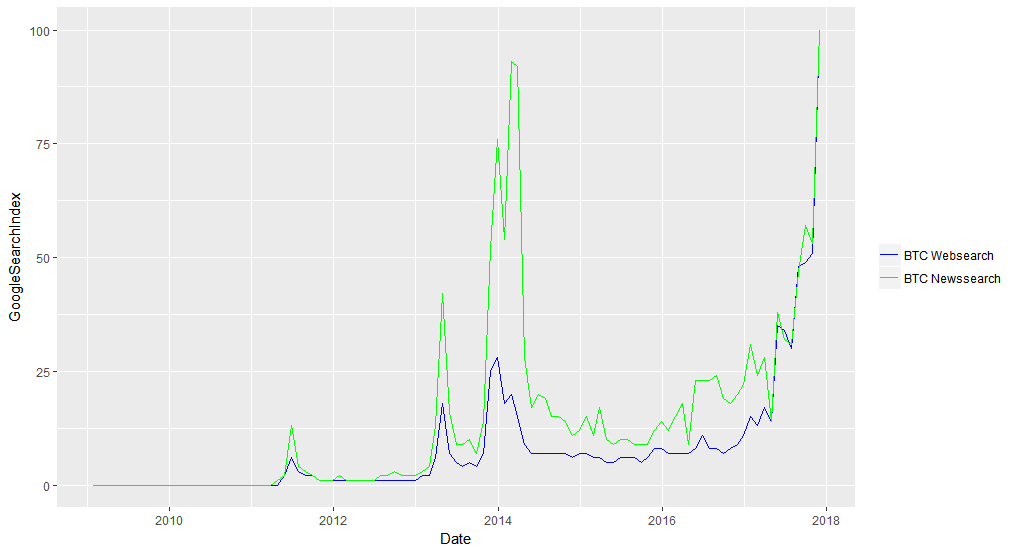
\includegraphics[width=\textwidth]{images/BTCpublicWithoutPrice}}
\caption{Google Websuchen und Newssuchen für "Bitcoin" im zeitlichen Verlauf}
\label{fig:PublicInterestBTC}
\end{figure}
Interpretiert man die Googlesuchen als Indikator für den Bekanntheitsgrad des Bitcoins, so lässt sich daraus schließen, dass die Währung bis 2011 sehr unbekannt und erst nach 2013 wirklich bekannt war. Zieht man nun den Bitcoinkurs heran (Listing \ref{list:PublicInterestBTC2}), so lässt sich ein Zusammenhang erkennen (Abbildung \ref{fig:PublicInterestBTC2}). 
\lstinputlisting[caption=Google Websuchen und Newssuchen für "Bitcoin" und Bitcoinkurs im zeitlichen Verlauf in R,label=list:PublicInterestBTC2]{../R/punlicInterestPlots/PublicInterestBTC2.R}
\begin{figure}[H]
\centering
\frame{
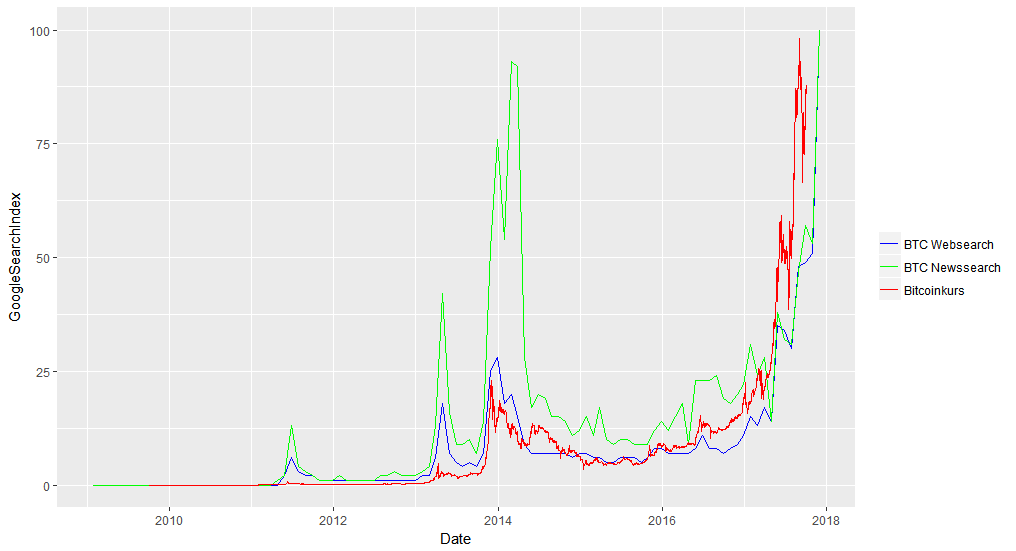
\includegraphics[width=\textwidth]{images/BTCpublicWithPrice}}
\caption{Google Websuchen und Newssuchen für "Bitcoin" im zeitlichen Verlauf}
\label{fig:PublicInterestBTC2}
\end{figure}
(Anzumerken ist, dass die historischen Kursdaten hier in keinem Verhältnis zur y-Achse stehen und nur der grafischen Darstellung dienen.)
Anders verhält es sich bei Ethereum (siehe Abbildung \ref{fig:PublicInterestETH}). Hier besteht schon vor dem offiziellen Start des Ethereumnetzwerks\citep{tual_ethereum_2015} ein gewisses Interesse.
\begin{figure}[H]
\centering
\frame{
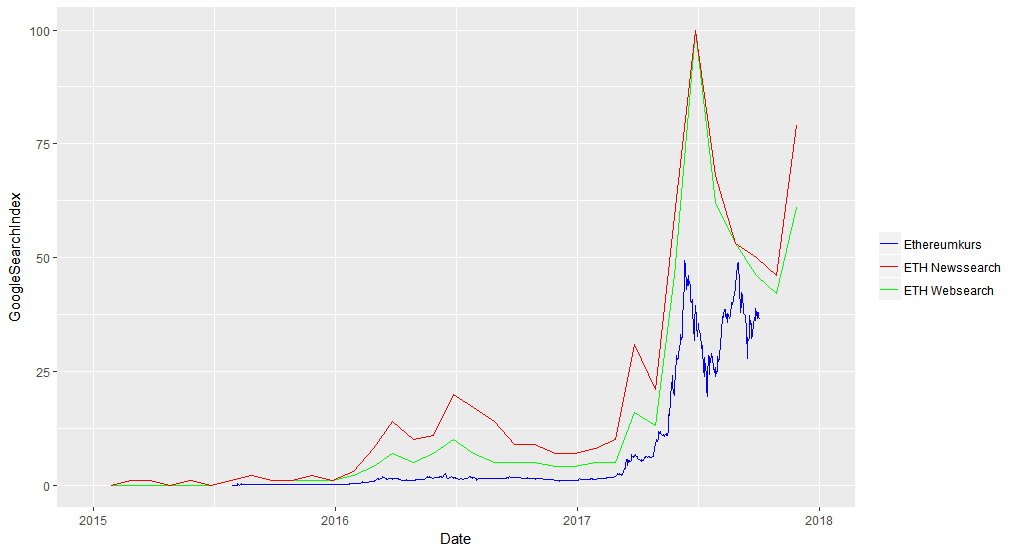
\includegraphics[width=\textwidth]{images/ETHpublicWithPrice}}
\caption{Google Websuchen und Newssuchen für "Ethereum" im zeitlichen Verlauf}
\label{fig:PublicInterestETH}
\end{figure}
Als Schlussfolgerung lässt sich daraus ableiten, dass es sehr unwahrscheinlich ist, dass Indikatoren wie Aktienindizes oder der Ölpreis den Kryptowährungskurs beeinflussen, wenn sie noch unbekannt ist. Deswegen empfiehlt sich für die Analyse der Zeitraum, seit die Währungen Bekanntheit erlangt haben. 

\begin{centering} \begin{longtable}[H]{|p{4,5cm}|p{12cm}|}
\hline
\textbf{Output} & \textbf{Beschreibung} \\ 
\hhline{==}
Data exploration report & Analyse des Bitcoinkurses erst ab 1.1.2011; des Ethereumkurses ab 30.7.2015\\
\hline
\caption{Output des Schrittes "Explore the Data"}
\end{longtable} \end{centering}

\subsection{Problemen mit den Daten und mögliche Lösungen (Verify Data Quality)}
Bei der Sicherung der Datenqualität fällt auf, dass die Daten oberflächlich eine hohe Qualität aufweisen. Beispielsweise sind alle Datensätze in USD angegeben und strukturiert. Sie enthalten pro Datei nicht viele Features und besitzen kaum lückenhafte Spalten. Jedoch sind einige Dinge zu beachten (siehe Tabelle \ref{tab:dataQual}).

\begin{centering} \footnotesize \begin{longtable}[H]{|p{7cm}|p{9cm}|}
\hline
\textbf{Problem} & \textbf{Lösung} \\ 
\hhline{==}
Die verschiedenen Datensätze haben unterschiedliche Datumsformate. Dies birgt Risiken beim Zusammenführen der Daten. & Vor dem Joinen der Daten müssten die Formate uniformiert werden. Dies kann beispielsweise mit der R-Methode \begin{lstlisting}
as.Date(data$DateColumn, format='%Y%m%d')
\end{lstlisting}
geschehen, solange das Datum in einem gültigen Format ist. \\ \hline
Beim Zusammensetzen der Datensätze entstehen Lücken, da einige Datensätze (z.B. Kryptowährungs-eigene Eigenschaften) sieben Observations pro Woche festhalten, Andere (z.B. Aktienindizes) nur fünf. Außerdem gibt es Datensätze mit Feiertagen (z.B. Neujahr) oder solche mit nur einer Observation pro Woche (z.B. STLFSI). & Azure ML Studio bietet das Experiment Item 'Clean Missing Data' an. Neben den Möglichkeiten, fehlende Daten mit dem Modus, Median oder Mittelwert auszufüllen, kann das Verfahren \gls{mice}\citep{azur_multiple_2011} oder die Probablilistic PCA\citep{tipping_probabilistic_1999} genutzt werden. \\ \hline
Durch die unterschiedlichen Formatierungen gibt es inkonsistente Separatoren (Komma, Semikolon, Tab), Dezimaltrennzeichen (Punkt, Komma) und Tausendertrennzeichen (Punkte, ohne Trennzeichen). & Vor dem Zusammenführen müssen die Separatoren und Trennzeichen untersucht und eventuell umgeändert werden. Dies kann mit Excel ('Speichern als...' oder Notepad++ ('Find and Replace') geschehen. Nach dem Joinen muss nachgeprüft werden. \\ \hline
Die Schwierigkeit für das Ethereumining wird im Datensatz ethereumDataset anfangs mit kleiner als 1 angeben. Dies ist per Definition unmöglich. & Entweder es handelt sich hier um einen undokumentierte Sonderfall zu Beginn des Netzwerks oder es ist ein Fehler im Datensatz. Trotz dieser Unstimmigkeit, ist die Tatsache insignifikant und kann vernachlässigt werden. \\ \hline
\caption{Data quality report des Schrittes "Verify data quality"}
\label{tab:dataQual}
\end{longtable} \end{centering}

\section{Data Preparation}\label{sec:p3}
\subsection{Inkludieren und Expludieren von Daten (Select Data)}
Die Datensätze sind nun gut beschrieben und es wurde auf Herausforderungen und Probleme hingewiesen. Die folgenden Punkte befassen sich damit, die richtigen Daten und Features weiter zu reduzieren ("Select Data"), sie zu reinigen ("Clean Data") und schließlich zum endgültigen Analyse-Datensatz zusammenfassen ("Construct Data", "Integrate Data" und "Format Data").
Ausgenommen der jetzt begründet ausgeschlossenen Daten, werden alle Vorgestellten zum bilden des \gls{model} genutzt. Tabelle \ref{tab:selecData} liefert einen Überblick.

In Punkt \ref{subsec:collection} wurde festgestellt, dass der Datensatz 'BTC \textunderscore Total \textunderscore Volume \textunderscore Daily \textunderscore Full' große Lücken enthält. Darüber hinaus enthält der Datensatz 'bitcoinDataset' ebenfalls die Anzahl der Bitcoins als Feature 'btc \textunderscore total \textunderscore bitcoins'. Ein stichprobenhafter Konsistenzcheck ergibt, dass die vorhanden Daten sich decken. Aus diesem Grund wird der Lückenhafte Datensatz exkludiert. 
'BTC \textunderscore Difficulty \textunderscore Daily \textunderscore Full' enthält wie 'bitcoinDataset' die Miningschwierigkeit (siehe Punkt \ref{sec:cryptocurrency2}). Obwohl der einzelne Datensatz minimal genauere Werte enthält, fällt die Wahl erneut auf das 'bitcoinDataset', da es Daten über eine längere Zeitspanne enthält. Genauso verhält sich bei 'BTC \textunderscore Transaction \textunderscore Number \textunderscore Fully \textunderscore Daily' und 'BTC \textunderscore Price \textunderscore Multiple \textunderscore Daily'. 
Analog wird bei den Ethereumdatensätzen vorgegangen. 'ETH \textunderscore Total \textunderscore Volume \textunderscore Daily \textunderscore Full' enthält die gleichen Daten wie 'ethereumDataset'. Allerdings um Faktor 100000 erhöht. Vermutlich handelt es sich hierbei um einen Konvertierungs- oder Kopierfehler, da das derzeit mögliche Maximum bei 100 Millionen Ether liegt \multicitep{buterin_lets_2016; hawksby-robinson_what_2017}. Die Werte für die Schwierigkeit und Anzahl der Transaktionen stimmen bei 'ETH \textunderscore Difficuly \textunderscore Daily \textunderscore Full' bzw. 'ETH \textunderscore Transaction \textunderscore Number \textunderscore Fully' mit 'ethereumDataset' genau überein. 
Der Bitcoinkurs soll vom 1.1.2011 an analysiert werden. Für einige Aktienindizes liegen für diese Zeit noch keine Daten vor. Um die über 50 Indizes auszudünnen, werden nur solche für das Machine Learning genutzt, für die Daten vorhanden sind. Dadurch wird versucht, Datenlücken zu vermeiden. Damit der Arbeitsaufwand reduziert wird, wird die Auswahl für die Analyse des Ethereumpreises übernommen. Die Google Trends Daten werden beibehalten. Anders verhält es sich bei den Wikipedia-Seitenaufrufen. Für die Bitcoinanalyse ist die Zeitspanne des Datensatzes zu kurz (es fehlen 4 1/2 Jahre: von 1.1.2011 bis 1.7.2015). Eine mögliche Korrelation (siehe Abbildung \ref{fig:WikiBTC}) zwischen Seitenaufrufen und Bitcoinkurs müsste gesondert untersucht werden. 
\begin{figure}[H]
\centering
\frame{
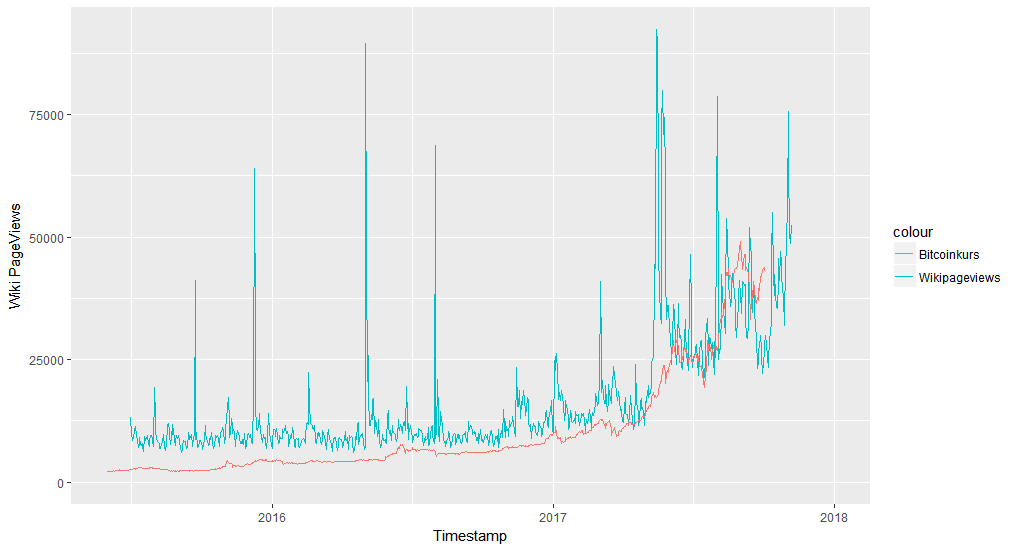
\includegraphics[width=\textwidth]{images/WikiPageBTC}}
\caption{Wikipedia Seitenaufrufe "Bitcoin" und der Bitcoinkurs im zeitlichen Verlauf}
\label{fig:WikiBTC}
\end{figure}
Für die Ethereumkursanalyse werden die Seitenaufrufe herangezogen, da sich die Daten zeitlich decken (siehe Abbildung \ref{fig:WikiETH}). (Erneut ist bei beiden Diagrammen der Kryptowährungskurs nur relativ dargestellt und nicht als absolute Größe.)
\begin{figure}[H]
\centering
\frame{
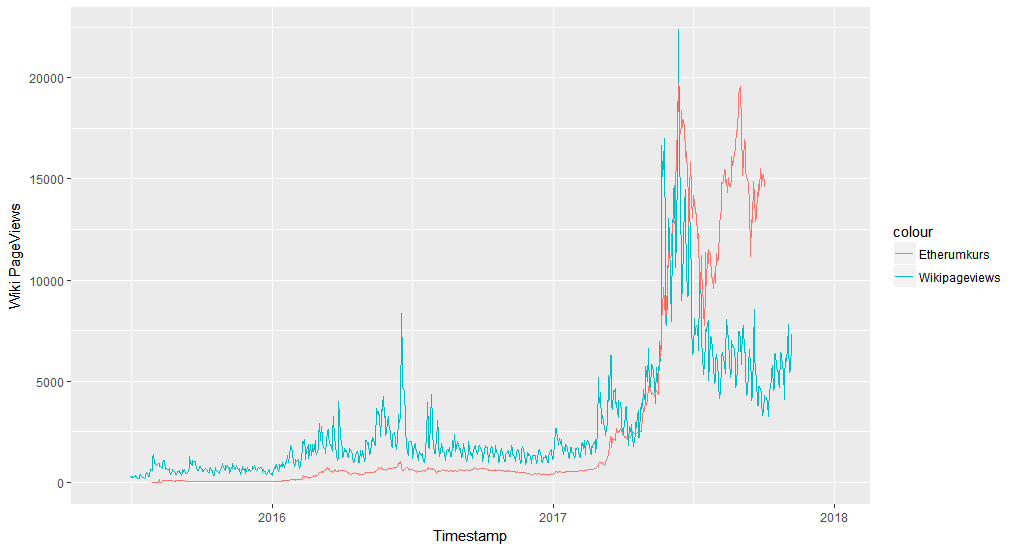
\includegraphics[width=\textwidth]{images/WikiPageETH}}
\caption{Wikipedia Seitenaufrufe "Ethereum" und der Ethereumkurs im zeitlichen Verlauf}
\label{fig:WikiETH}
\end{figure}
Obwohl für den STLFSI nur wöchentlich - nicht täglich - berechnet wird, wird er beibehalten. Bei den Währungen wird nur der Kurs INR/USD exkludiert, da hier nur Daten ab dem 9.9.2014 vorliegen. Alle Daten zu natürlichen Ressourcen (Gold, Silber, Öl) werden inkludiert.
Dem Datensatz 'ETH \textunderscore Price \textunderscore Volume \textunderscore Full \textunderscore Daily' fehlt die erste Woche an Daten, ist sonst aber reicher an Informationen über den Ethereum/USD-Kurs als das 'ethereumDataset', da es nicht nur den Durchschnittspreis eines Tages enthält, sondern sowohl den ersten und letzten Kurs in einem 24-Stunden-Fenster, als auch den Höchsten und den Niedrigsten. Dem 'BTC \textunderscore Price \textunderscore Volume \textunderscore Full \textunderscore Daily' hingegen fehlt das erste halbe Jahr an Daten und weist erst ab Ende (18.12.) 2011 keine Lücken mehr auf. In allen Datensätzen (Aktienindizes, Währungen, natürliche Ressourcen) wird das Feature '\%Change' gestrichen, da in \ref{subsec:describe} festgestellt wurde, dass es redundant ist.
abcnews \textunderscore Date \textunderscore Text wird beibehalten. 
Auch wenn die Datensätze an dieser Stelle aussortiert werden, war ihre Beschreibung keine Verschwendung. Sie hat dazu beigetragen, das Domainwissen zu vertiefen und die Plausibilität der Daten zu prüfen.

\begin{centering} \footnotesize \begin{longtable}[H]{|p{12cm}|p{1,5cm}|p{1,5cm}|}
\hline
\textbf{Datensatz} & \textbf{Inkludiert} & \textbf{Exkludiert} \\ 
\hhline{===}
BTC \textunderscore Total \textunderscore Volume \textunderscore Daily \textunderscore Full & & X \\ \hline
BTC \textunderscore Difficulty \textunderscore Daily \textunderscore Full & & X \\ \hline
BTC \textunderscore Transaction \textunderscore Number \textunderscore Fully \textunderscore Daily & & X \\ \hline
BTC \textunderscore Price \textunderscore Multiple \textunderscore Daily & & X \\ \hline
ETH \textunderscore Total \textunderscore Volume \textunderscore Daily \textunderscore Full & & X \\ \hline
ETH \textunderscore Difficuly \textunderscore Daily \textunderscore Full & & X \\ \hline
ETH \textunderscore Transaction \textunderscore Number \textunderscore Fully \textunderscore Daily & & X \\ \hline
google \textunderscore Trends \textunderscore BTC \textunderscore Websearch & X & \\ \hline
google \textunderscore Trends \textunderscore ETH \textunderscore Websearch & X & \\ \hline
google \textunderscore Trends \textunderscore BTC \textunderscore Newssearch & X & \\ \hline
google \textunderscore Trends \textunderscore ETH \textunderscore Newssearch & X & \\ \hline
Wiki \textunderscore Page \textunderscore Views \textunderscore BTC &  & X \\ \hline
Wiki \textunderscore Page \textunderscore Views \textunderscore ETH & X & \\ \hline
abcnews \textunderscore Date \textunderscore Text  & X & \\ \hline
FTXIN9, PSI20, AEX, BFX, XU100, BVSP, VIX, CSE, GDAXI, DJI, FTSE, FTMIB, HSI, IBEX, MXX, JKSE, KSE, KS11, MCX, IXIC, NSEI, N225, OMXC20, OMXS30, IRTS, SPX, AXJO, GSPTSE, SSEC, SSMI, TA35, TASI, TRX50CAP, US2000, WIG20 & X & \\ \hline
ATX, BSESN, BUX, NZDOW, DJSH, STOXX50E, STI, HNX30, PSI, SETI, SZSC1, TWII & & X \\ \hline
STLFSI & X & \\ \hline
CNY \textunderscore USD \textunderscore history & X & \\ \hline
JPY \textunderscore USD \textunderscore history & X & \\ \hline
EUR \textunderscore USD \textunderscore history & X & \\ \hline
GBP \textunderscore USD \textunderscore history & X & \\ \hline
INR \textunderscore USD \textunderscore history & & X \\ \hline
BRL \textunderscore USD \textunderscore history & X & \\ \hline
gold \textunderscore history & X &  \\ \hline
silver \textunderscore history  & X &  \\ \hline
oil \textunderscore brent \textunderscore history  & X &  \\ \hline
oil \textunderscore wti \textunderscore history  & X &  \\ \hline
ETH \textunderscore Price \textunderscore Volume \textunderscore Full \textunderscore Daily & X & \\ \hline
BTC \textunderscore Price \textunderscore Volume \textunderscore Full \textunderscore Daily & & X \\ \hline
bitcoinDataset & X & \\ \hline
ethereumDataset & X & \\ \hline
\caption{Inkludierte und exkludierte Datensätze für die Analyse}
\label{tab:selecData}
\end{longtable} \end{centering}

\subsection{Aufbereitung der Daten (Clean, Construct, Integrate, Format Data)}

Die Schritte 'Clean Data', 'Construct Data', 'Integrate Data' und 'Format Data' gehen Hand in Hand. Deswegen werden die Punkte zusammengefasst. Bei der tatsächlichen Durchführung wurden die Schritte iterativ und inkrementell durchlaufen. \par
Die Menge aller Daten für die Untersuchung ist heterogen. Es existieren jedoch Blöcke (z.B. alle Währungskurse oder alle natürlichen Ressourcen), die innerhalb eine homogene Struktur aufweisen. Aus diesem Grund ist es ratsam, zuerst die homogenen Daten zusammenzufassen und diese großen Blöcke dann zusammenzufügen. Durch dieses Buttom-Up-Zusammensetzen wird die Integration vereinfacht.
Das Vorgehen ist dabei folgendes:
\begin{itemize}
\item Die einzelnen Datensätze werden so bearbeitet, dass sie für die Zusammenführung in ihren Block bereit sind.
\item Die bearbeiteten Daten werden ihrem Datenblock hinzugefügt. Das Ergebnis wird untersucht und eventuelle Unreinheiten beseitigt.
\item Alle Blöcke werden in einen abschließenden Datensatz integriert. Dieser wird wiederum inspiziert und bereinigt.
\end{itemize}
Nachfolgend wird das Bereinigen und Zusammensetzten beschrieben. Zuerst werden die Aktienindizes bearbeitet (Listing \ref{list:indicesR}) und gejoint (Abbildung \ref{fig:indicesAzure_1}). 
\lstinputlisting[caption=Aufbereiten der Indizes-Datensätze,label=list:indicesR]{../R/processIndexSets/processDataSet_Indices.R}
\begin{figure}[H]
\centering
\frame{
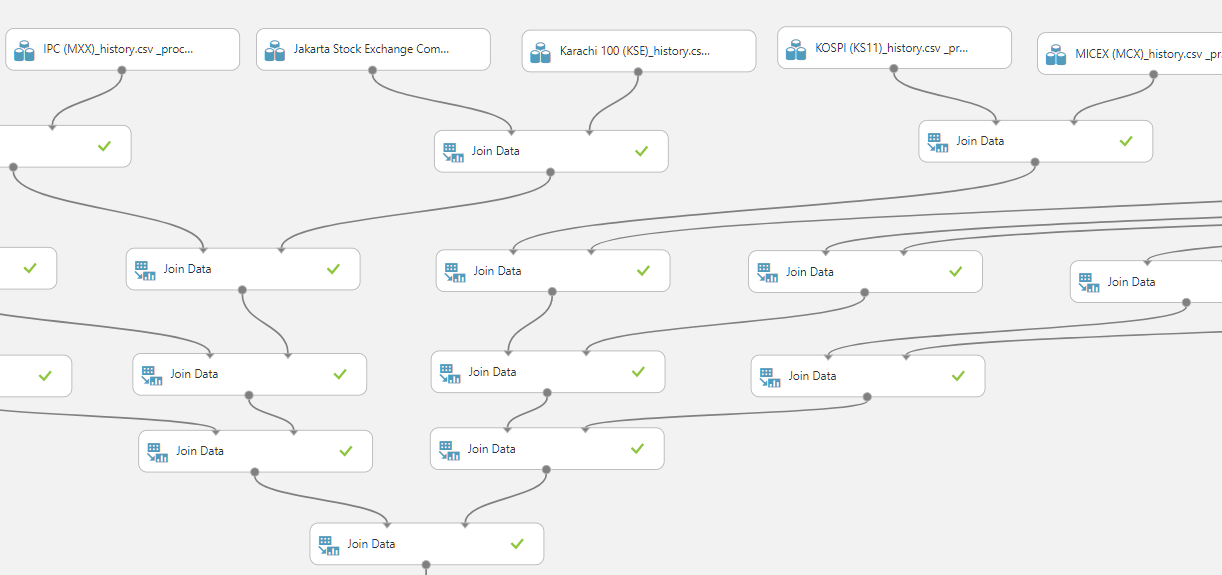
\includegraphics[width=\textwidth]{images/indicesAzure_1}}
\caption{Zusammenführen der Aktienindizes in Azure Machine Learning Studio}
\label{fig:indicesAzure_1}
\end{figure}
Daraufhin werden sie nachbearbeitet (die Beschreibung bezieht sich auf Abbildung \ref{fig:indicesAzure_2}): In jedem Ursprungsdatensatz existiert eine Spalte, die die Zeilen durchnummeriert. Dies diente zum beheben von Fehlern und wird nun entfernt (1. Select Columns in Dataset). Ebenso enthält das Ergebnis noch 35 Datums-Spalten (von jedem Ursprungsdatensatz eine). Diese werden bis auf Eine entfernt (2. Select Columns in Dataset und Edit Metadata).
\begin{figure}[H]
\centering
\frame{
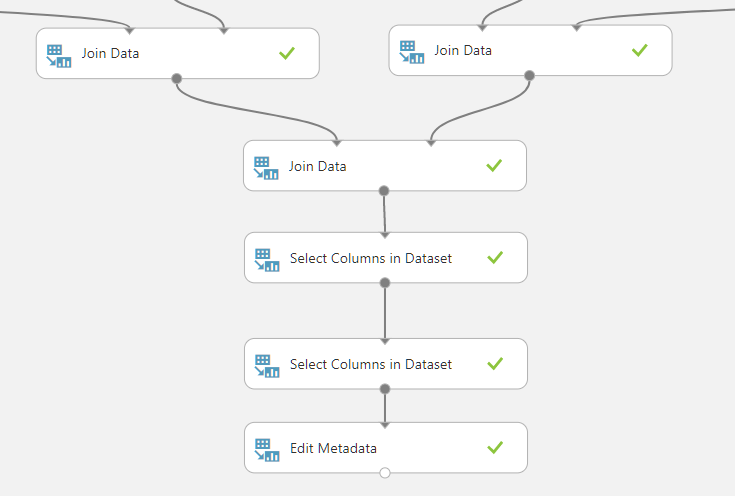
\includegraphics[width=\textwidth]{images/indicesAzure_2}}
\caption{Nachbearbeiten des Ergebnisdatensatzes in Azure Machine Learning Studio}
\label{fig:indicesAzure_2}
\end{figure}
Analog werden die natürlichen Ressourcen zu einem Datenblock zusammengefasst. Ähnlich wird mit den Währungskursen vorgegangen. Die Verarbeitung in R ist jedoch einfacher, da sie keine Tausendertrennzeichen, keine pseudo-numerischen Werte und keine Lücken enthalten. 
Spezieller ist der Datensatz 'abcnews \textunderscore Date \textunderscore Text' (siehe Abbildung \ref{fig:abcAzure1}). Er wird mit dem Experiment Item 'Preprocess Text' vorbearbeitet, nachdem alte Überschriften (vor dem 1.1.2011) entfernt wurden (Execute R Script; siehe Listing \ref{list:abcold} Zeile 6). 
\begin{figure}[H]
\centering
\frame{
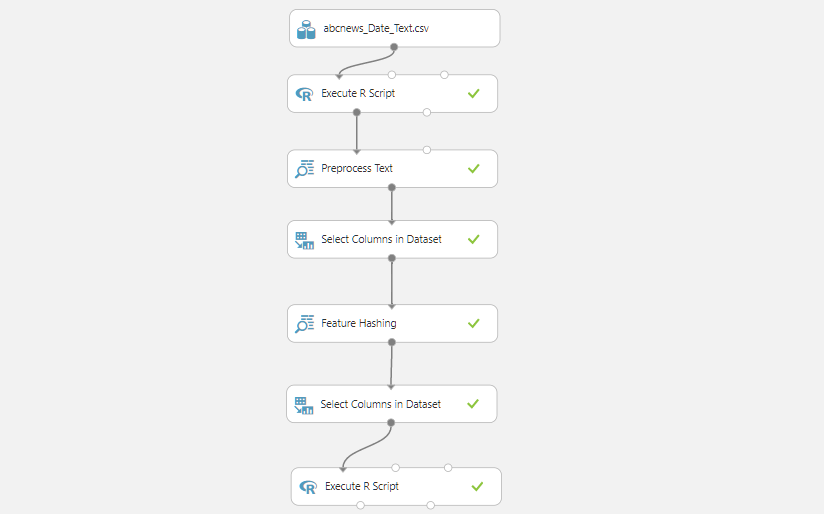
\includegraphics[width=\textwidth]{images/abcAzure1}}
\caption{Feature Hashing der abcnews in Azure Machine Learning Studio}
\label{fig:abcAzure1}
\end{figure}
\lstinputlisting[caption=Entfernen der alten Überschriften,label=list:abcold]{../R/abc/abcold.R}
Das Preprocessing führt unter anderem eine Lemmatisierung durch und entfernt Zahlen und Sonderzeichen. Anschließend wird ein Feature Hashing durchgeführt. Dabei handelt es sich um die Überführung von Texttupeln in Zahlwerte, damit eine Verarbeitung durch Computer möglich wird. Für jede Überschrift existiert eine einzelne Zeile im Datensatz. Diese werden mit dem R-Script in Listing \ref{list:abcHashed} in Azure aggregiert.
\lstinputlisting[caption=Aggregieren der Hashing-Ergebnisse,label=list:abcHashed]{../R/abc/abcHashed.R}
Zuletzt werden noch die Google News- und Websuchen zusammengefasst. Der abschließende Data cleaning report ist in Tabelle \ref{tab:selecData} zu finden.

\begin{centering} \begin{longtable}[H]{|p{4cm}|p{8cm}|p{4cm}|}
\hline
\textbf{Problem} & \textbf{Lösung} & \textbf{Werkzeug} \\
\hhline{===} 
unterschiedliche Datumsformate & Zuerst werden die Daten in Text und anschließend mit dem Packet 'anytime' in R konvertiert. & R + Package 'anytime' (siehe Listing \ref{list:indicesR} Zeile 37) \\ \hline
Lücken durch joinen der Daten & Es handelt sich um 'Missing not at random'-Fehler (MNAR)\citep[S.~553]{graham_missing_2009}. Das bedeutet, dass die Lücken absichtlich sind (weil an diesen Tagen nicht gehandelt wird). Da es kein statistisches Verfahren zum schließen solcher Lücken gibt, werden sie beibehalten. \citep[S.~1109]{leonhart_dorsch_2014} & \\ \hline
unterschiedliche Separatoren, Trennzeichen etc. & Die Daten werden mit Excel von '.tsv' in '.csv' konvertiert. Eine programmatische Änderung oder 'Find and Replace' ist schwer, da es einen Tab als Trennzeichen zwischen Tag, Monat und Jahr gibt. Kommas als Tausendertrennzeichen werden entfernt. & Excel 'Save As...' und R-Methode 'gsub' (siehe Listing \ref{list:indicesR} Zeilen 30-34) \\ \hline
pseudo-numerische Werte (z.B. "1.5M" oder "0.07k") & Bei betroffenen Werten wird der Buchstabe entfernt und die Zahl mit dem entsprechenden Wert multipliziert (z.B. $ 1.3 \times 1000 $ für 1.3K) & R-Methoden 'gsup' und 'grepl', sowie mathematische Operationen (siehe Listing \ref{list:pseudonumeric})\\ \hline
Fehlende Werte & Fehlende Werte im Volumen werden als '-' angegeben, nicht als 'Nichts'. Durch ersetzen des '-' in R wird das Problem behoben. & R: Listing \ref{list:indicesR} Zeile 45 \\ \hline
\caption{Data cleaning report}
\label{tab:selecData}
\end{longtable} \end{centering}
\lstinputlisting[caption=Konvertierung von pseudo-numerischen Werten,label=list:pseudonumeric]{../R/pseudonumeric.R}
Der Schritt 'Construct data' enthält die Möglichkeit, neue Features hinzuzufügen. Hier ist kein Bedarf dafür. Außerdem handelt es sich teilweise schon um stark aggregierte Features, wie den STLFSI (siehe \ref{subsec:assesTheSituation}). Damit sind die Konvertierungen, Formatierungen und Zusammenführungen der Datenblöcke abgeschlossen. Die Ergebnisse sind in den Tabellen \ref{tab:constructData} und \ref{tab:integrateData} festgehalten.

\begin{centering} \begin{longtable}[H]{|p{6cm}|p{9,5cm}|}
\hline
\textbf{Output} & \textbf{Beschreibung}\\
\hhline{==}
Hashed \textunderscore news & Die abcsnews nach dem Feature Hashing und der Aggregation. \\ \hline
\caption{Output: Generated records}
\label{tab:constructData}
\end{longtable} \end{centering}
\begin{centering} \begin{longtable}[H]{|p{6cm}|p{9,5cm}|}
\hline
\textbf{Output} & \textbf{Beschreibung}\\
\hhline{==}
Joined \textunderscore Indices & Alle Aktienindizes in einem Datensatz. \\ \hline
Joined \textunderscore Currencies & Alle Währungen in einem Datensatz.  \\ \hline
Joined \textunderscore Resources & Alle natürlichen Ressourcen in einem Datensatz. \\ \hline
Joined \textunderscore Public & Google Suchen und Google Newssuchen in einem Datensatz. \\ \hline
\caption{Output: Merged data}
\label{tab:integrateData}
\end{longtable} \end{centering}
Syntaktische Änderungen an den Datensätzen, also verändern der Spaltenreihenfolgen oder der Spaltenbezeichnungen sind Teil des Schrittes 'Format data'. Es kann beispielsweise in einem eingesetzten Werkzeug notwendig sein, dass die erste Spalte einer Tabelle ein eindeutiger Schlüssel sein muss \citep[S.~46]{chapman_crisp-dm_2000}. Obgleich dieser Fall hier nicht eintritt, werden syntaktische Änderungen vorgenommen: Wie oben bereits erwähnt, entstehen beim Zusammenführen der Tabellen doppelte Spalten. Werden zwei Tabellen gejoint, so existieren zwei Datumsspalten, die die gleichen Werte beinhalten (rechte Datumsspalte und linke Datumsspalte). Diese Redundanzen werden entfernt. Außerdem wird die beibehaltene Spalte in 'Date' umbenannt.\par
Alle erzeugten Blöcke und einzelnen Datensätze werden nun im Azure Machine Learning Studio zu einem Datensatz zusammengefasst. Für das Machine Learning werden aus diesem die benötigten Spalten für BTC bzw. ETH ausgewählt. Da das Joinen wie bisher verläuft, wird auf eine extra Beschreibung von Abbildung \ref{fig:azureFinalSet} verzichtet.
\begin{figure}[H]
\centering
\frame{
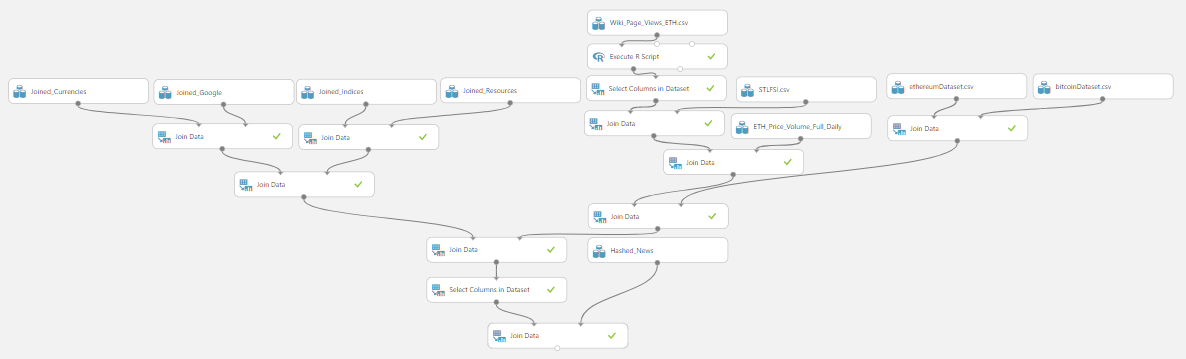
\includegraphics[width=\textwidth]{images/azureFinalSet}}
\caption{Erzeugen des finalen Datensatzes für das Machine Learning}
\label{fig:azureFinalSet}
\end{figure}
Der letzte Schritt vor dem Machine Learning ist das Auswählen des Analysezeitraums und das bereinigen fehlender Daten (siebe Abbildung \ref{fig:azureDateAndCleaning}).
\begin{figure}[H]
\centering
\frame{
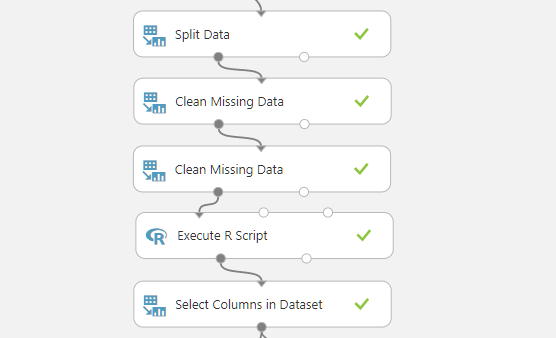
\includegraphics[width=\textwidth]{images/azureDateAndCleaning}}
\caption{Auswahl des Analysezeitraums und bereinigen fehlender Daten in Azure Machine Learning Studio}
\label{fig:azureDateAndCleaning}
\end{figure}
Um nur die Zeilen zur Analyse zu benutzen, die im ausgewählten Zeitintervall (siehe Punkt \ref{subsec:explore}) liegen, wird das Datenset noch aufgesplittet (Experiment Item 'Split Data' mit Relative Expression \textbackslash "Date" >= 2011-01-01T00:00:00 für BTC und \textbackslash "Date" >= 2015-07-30T00:00:00 für ETH). Daraufhin werden mit dem Item 'Clean Missing Data (Probabilistic PCA))' fehlende Daten ersetzt, die nicht unter die Kategorie MNAR fallen. Bei neun Spalten ist dies nicht möglich (keine Fehlermeldung in Azure Machine Learning; vermutlich zu wenige Werte für Probabilistic PCA). Diese werden mit einem erneuten 'Clean Missing Data (Remove entire column)' entfernt. Als Abschluss wird mit dem R-Script in Listing \ref{list:AzureIncrease} eine neue Spalte angefügt, die angibt, ob der Kurs zum Vortag gestiegen ist (Wert: 1) oder nicht (Wert: 0). Dieser wird im Nachfolgenden als Vorhersagewert genutzt.
\lstinputlisting[caption=Hinzufügen und Popularisieren der Spalte "increase" in Azure Machine Learning Studio,label=list:AzureIncrease]{../R/AzureIncrease.R}


\section{Modeling}\label{sec:p4}
\subsection{Auswahl von Klassifizierungs- und Regressionsalgorithmen (Select the Modeling Technique)}
Wie in Punkt \ref{subsec:goals} gefordert, wird einerseits versucht, einen Wert für den Kurs vorherzusagen (mit Hilfe von Regressionen) und andererseits, ob der Kurs steigt oder nicht (Two-Class classification). In beiden Fällen handelt es sich um Supervised Learning, da für jeden Input ein Output vorhanden ist (siehe Punkt \ref{subsec:sl}).
In Azure verfügbare Two-Class classification Algorithmen sind:
\begin{itemize}
\item Two-Class Support Vector Machine
\item Two-Class Neural Network
\item Two-Class Logistic Regression
\item Two-Class Locally-Deep Support Vector Machine
\item Two-Class Decision Jungle
\item Two-Class Decision Forest
\item Two-Class Boosted Decision Tree
\item Two-Class Bayes Point Machine
\item Two-Class Averaged Perceptron
\end{itemize}
Bei den Regressionen sind es:
\begin{itemize}
\item Bayesian Linear Regression
\item Boosted Decision Tree Regression
\item Decision Forest Regression
\item Fast Forest Quantile Regression (*)
\item Linear Regression (*)
\item Neural Network Regression
\item Ordinal Regression (*)
\item Poisson Regression (*)
\end{itemize}
Ausgeschlossen (mit * gekennzeichnet) werden Ordinal Regression (nur geeignet, um Rangfolgen aufzustellen), Poisson Regression (nur geigten, um vorherzusagen, wie oft etwas passiert), Linear Regression (nur für sehr simple Modelle) und Ordinal Regression (zwar geeignet, nutzt aber andere Metriken und ist nicht vergleichbar).
Die Algorithmen besitzen konfigurierbare Parameter. Die Güte der erzeugten Modelle hängt unter anderem von diesen einstellbaren Werten ab. Azure bietet die Möglichkeit, die Parameter automatisch zu optimieren. Dazu wird das Experiment Item 'Tune Model Hyperparameter' eingesetzt. Es verbessert das Ergebnis des Models hinsichtlich eines bestimmten Wertes (Genauigkeit, Präzision etc.). Im vorliegenden Fall werden als Zielparameter die Metriken aus den Data Mining Goals (Punkt \ref{subsec:goals}) gewählt:
F1-Score für Klassifikationen und Bestimmtheitsmaß (Coefficient of determination) für die Regressionen.

\subsection{Festlegung des Verhältnis von Trainings- und Testdaten (Generate Test Design)}
Es muss überlegt werden, in welchem Verhältnis die zu analysierenden Daten aufgeteilt werden (Trainingsdaten : Testdaten). Es gibt kein allgemeingültiges, optimales Verhältnis. In der Praxis sind jedoch Verhältnisse wie 70:30 oder 80:20 üblich. Es existieren auch andere Ansätze, die wiederum auf Algorithmen basieren \citep{crowther_method_2005}. Beachtet werden muss jedoch, dass nicht einfach obere und untere Hälfte des Datensatzes genutzt werden, sondern die Aufteilung nach dem Zufallsprinzip geschieht. Da das Experiment Item 'Tune Model Hyperparameter' eingesetzt wird, gibt es die Möglichkeit, ein zusätzliches Validation Dataset zu nutzen. Das für diese Analyse gewählte Verhältnis (Training 56 : Validierung 14 : Test 30) ist in Abbildung \ref{fig:ratio} visualisiert.
\begin{figure}[H]
\centering
\frame{
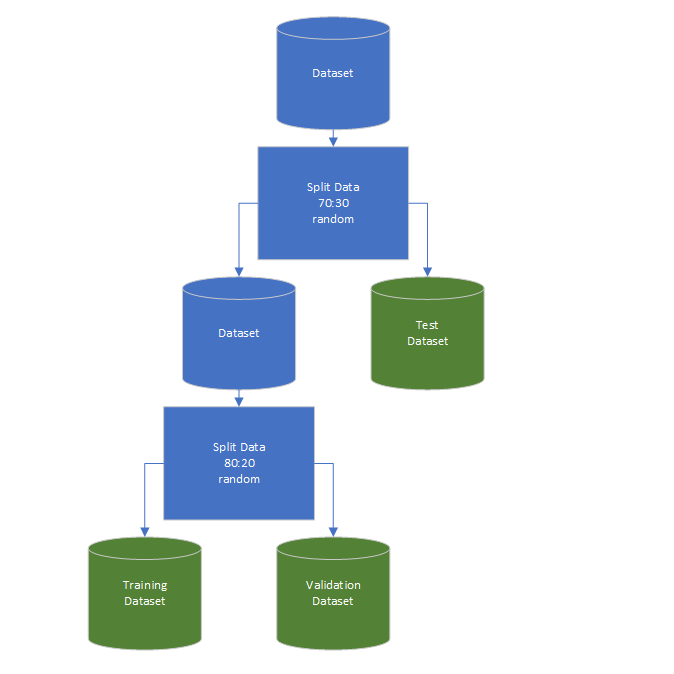
\includegraphics[width=12cm]{images/ratio}}
\caption{Verhältnis der Aufteilen in Trainings-, Test- und Validierungsdatensatz (Output Testdesign)}
\label{fig:ratio}
\end{figure}

\subsection{Durchführung des Machine Learning (Build the Model)}
Nachdem alle Vorbereitungen abgeschlossen sind, wird jetzt das eigentliche Machine Learning durchgeführt. Dazu werden vier Experimente in Azure Machine Learning Studio modelliert. Je eines für:
\begin{itemize}
\item die Kurspreisvorhersage für ETH (Regression für ETH),
\item die Kurspreisvorhersage für BTC (Regression für BTC),
\item die Vorhersage, ob der ETH Kurs steigt (Two-class classification für ETH) und
\item die Vorhersage, ob der BTC Kurs steigt (Two-class classification für BTC).
\end{itemize}
Die Experimente gleichen sich sehr, deswegen sind hier nur die Kurspreisvorhersage für ETH (Abbildung \ref{fig:azureETHReg}) und die Klassifikation für BTC (Abbildung \ref{fig:azureBTCClass}) abgebildet.

\begin{figure}[H]
\centering
\frame{
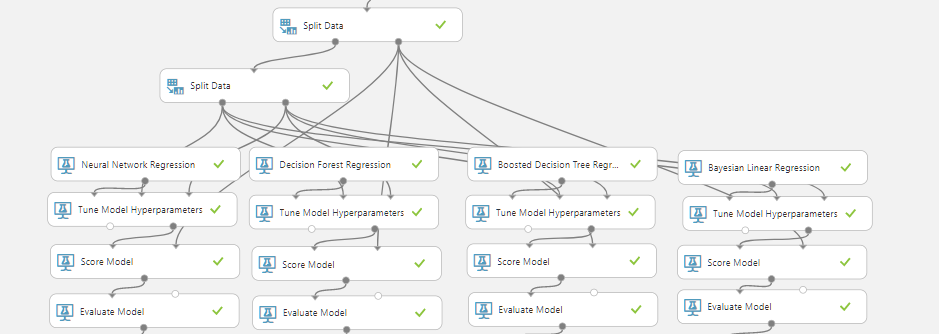
\includegraphics[width=\textwidth]{images/azureETHReg}}
\caption{Ethereum Regressionen in Azure Machine Learning Studio}
\label{fig:azureETHReg}
\end{figure}

\begin{figure}[H]
\centering
\frame{
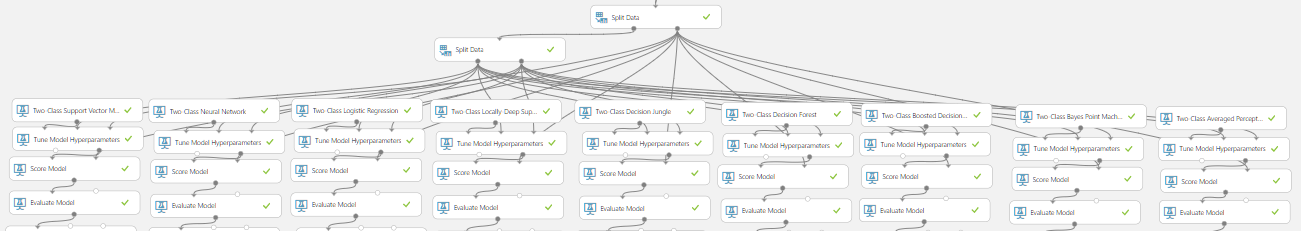
\includegraphics[width=\textwidth]{images/azureBTCClass}}
\caption{Bitcoin Klassifikation in Azure Machine Learning Studio}
\label{fig:azureBTCClass}
\end{figure}

Mit den zwei 'Split Data' Experiment Items wird der Analysedatensatz, wie im vorherigen Punkt spezifiziert, in Trainings-, Validierungs- und Testdaten aufgeteilt. Zu sehen ist auch das Item 'Tune Model Hyperparameter (entire grid)', das sowohl das Training des Models, als auch das optimieren der Algorithmenparameter übernimmt (deshalb an dieser Stelle kein Output "Parameter Settings" wie im Referenzmodell verlangt). Die Option 'entire grid' beim Verbessern der Parameter ist eine inperformante Option, die aber sehr genau arbeitet. Dies ist verkraftbar, da die Gesamtlaufzeit des Experiments 30 Minuten nicht deutlich überschreitet.

\subsection{Betrachtung der Ergebnisse (Assess the Model)}
Ein Durchlauf liefert folgende Ergebnisse:

\begin{table}[H]
\centering
\begin{tabular}{|p{5cm}|p{1,5cm}|p{1,5cm}|p{1,5cm}|p{1,5cm}|p{1,5cm}|}
\hline
\textbf{Algorithmus} & \textbf{F1-Score} & \textbf{Accuracy} & \textbf{Precision} & \textbf{Recall} & \textbf{AUC}\\ 
\hhline{======}
Two-Class Support Vector Machine & 0.565445 & 0.538889 & 0.568421 & 0.562500 & 0.552703 \\ \hline
Two-Class Neural Network & 0.685259 & 0.561111 & 0.554839 & 0.895833 & 0.571181 \\ \hline
Two-Class Logistic Regression & 0.559585 & 0.527778 & 0.556701 & 0.562500 & 0.568204 \\ \hline
Two-Class Locally-Deep Support Vector Machine & 0.547264 & 0.494444 & 0.52381 & 0.572917 & 0.517361 \\ \hline
Two-Class Decision Jungle & 0.698413 & 0.577778 & 0.564103 & 0.916667 & 0.553571 \\ \hline
Two-Class Decision Forest & 0.556818 & 0.566667 & 0.6125 & 0.510417 & 0.573289 \\ \hline
Two-Class Boosted Decision Tree & 0.514620 & 0.538889 & 0.586667 & 0.458333 & 0.570188 \\ \hline
Two-Class Bayes Point Machine & 0.684211 & 0.533333 & 0.535294 & 0.947917 & 0.595982 \\ \hline
Two-Class Averaged Perceptron & 0.522727 & 0.533333 & 0.575000 & 0.479167 & 0.573289 \\ \hline
\end{tabular}
\caption{Ergebnisse des Machine Learning: Ethereum Two-class Classification}
\label{tab:ETH2}
\end{table}

\begin{table}[H]
\centering
\begin{tabular}{|p{5cm}|p{1,5cm}|p{1,5cm}|p{1,5cm}|p{1,5cm}|p{1,5cm}|}
\hline
\textbf{Algorithmus} & \textbf{F1-Score} & \textbf{Accuracy} & \textbf{Precision} & \textbf{Recall} & \textbf{AUC}\\ 
\hhline{======}
Two-Class Support Vector Machine & 0.662937 & 0.552045 & 0.578049 & 0.777049 & 0.499951 \\ \hline
Two-Class Neural Network & 0.706199 & 0.594796 & 0.599542 & 0.859016 & 0.612805 \\ \hline
Two-Class Logistic Regression & 0.623946 & 0.585502 & 0.642361 & 0.606557 & 0.597031 \\ \hline
Two-Class Locally-Deep Support Vector Machine & 0.647555 & 0.611524 & 0.666667 & 0.629508 & 0.643130 \\ \hline
Two-Class Decision Jungle & 0.659236 & 0.602230 & 0.640867 & 0.678689 & 0.639724 \\ \hline
Two-Class Decision Forest & 0.656958 & 0.605948 & 0.648562 & 0.665574 & 0.650770 \\ \hline
Two-Class Boosted Decision Tree & 0.668750 & 0.605948 & 0.638806 & 0.701639 & 0.649595 \\ \hline
Two-Class Bayes Point Machine & 0.734082 & 0.604089 & 0.592742 & 0.963934 & 0.583691 \\ \hline
Two-Class Averaged Perceptron & 0.566957 & 0.537175 & 0.603704 & 0.534426 & 0.564160 \\ \hline
\end{tabular}
\caption{Ergebnisse des Machine Learning: Bitcoin Two-class Classification}
\label{tab:BTC2}
\end{table}

\begin{table}[H]
\centering
\begin{tabular}{|p{4cm}|p{1,7cm}|p{1,7cm}|p{1,7cm}|p{1,7cm}|p{1,7cm}|}
\hline
\textbf{Algorithmus} & \textbf{$ R^2 $} & \textbf{MAE} & \textbf{RMSE} & \textbf{RAE} & \textbf{RSE}\\ 
\hhline{======}
Neural Network Regression & -0.232605 & 69.99189 & 124.834987 & 0.737855 & 1.232605 \\ \hline
Boosted Decision Tree Regression & 0.999326 & 1.372442 & 2.918441 & 0.014468 & 0.000674 \\ \hline
Decision Forest Regression & 0.994616 & 3.514041 & 8.250093 & 0.037045 & 0.005384 \\ \hline
Bayesian Linear Regression & 0.999994 & 0.206625 & 0.272996 & 0.002178 & 0.000006 \\ \hline
\end{tabular}
\caption{Ergebnisse des Machine Learning: Ethereum Regression}
\label{tab:ETHREg}
\end{table}

\begin{table}[H]
\centering
\begin{tabular}{|p{4cm}|p{1,7cm}|p{1,7cm}|p{1,7cm}|p{1,7cm}|p{1,7cm}|}
\hline
\textbf{Algorithmus} & \textbf{$ R^2 $} & \textbf{MAE} & \textbf{RMSE} & \textbf{RAE} & \textbf{RSE}\\ 
\hhline{======}
Neural Network Regression & -0.105524 & 496.619518 & 717.756528 & 1.225332 & 1.105524 \\ \hline
Boosted Decision Tree Regression & 0.995827 & 10.095783 & 44.099144 & 0.02491 & 0.004173 \\ \hline
Decision Forest Regression & 0.995791 & 13.301142 & 44.290157 & 0.032819 & 0.004209 \\ \hline
Bayesian Linear Regression & 0.999946 & 2.273447 & 5.032831 & 0.005609 & 0.000054 \\ \hline
\end{tabular}
\caption{Ergebnisse des Machine Learning: Bitcoin Regression}
\label{tab:BTCReg}
\end{table}

Betrachtet man zuerst die beiden Regressionen (Tabellen \ref{tab:ETHREg} und \ref{tab:BTCReg}), so fällt auf, dass $ R^2 $ sehr hoch ist (Maximum ist $ R^2 = 1 $). Auf den ersten Blick zeugt das von einer nahezu perfekten Kurspreisvorhersage (Anmerkung: Ein $ R^2 $ von -0.105524 entspricht  $ R^2 = 1 - 0.105524 = 0.894476 $ ). Untersucht man das Ergebnis genauer, so sieht man, dass die vorhergesagten Werte sehr nahe an den Tatsächlichen liegen (siehe Tabelle \ref{tab:scoredReal}).
\begin{table}[H]
\centering
\begin{tabular}{|p{4cm}|p{4cm}|}
\hline
\textbf{Vorhergesagter Ethereumpreis in USD} & \textbf{tatsächlicher Preis in USD}\\ 
\hhline{==}
44.4758 & 44.16 \\ \hline
11.3525 & 11.41 \\ \hline
306.6813 & 306.72 \\ \hline
5.2086 & 5.38 \\ \hline
\end{tabular}
\caption{Ausschnitt des Ergebnisses der Vorhersage des Ethereumkurses mit einer Bayesian Linear Regression (nicht chronologisch; auf vier Nachkommastellen gerundet)}
\label{tab:scoredReal}
\end{table}
Bei der Beschreibung der Bewertungsmetriken in Punkt \ref{subsec:goals} wurde jedoch darauf hingewiesen, dass große Werte für $ R^2 $ misstrauisch machen sollten. Dieses Phänomen kann mehre Gründe haben. Hier liegen folgende Vermutungen vor:
\begin{itemize}
\item Es liegt ein Fall von Überanpassung (engl. overfitting) vor. "Ein überangepasstes Modell [...] ist zu kompliziert für die [darunterliegenden] Daten"\citep[eigene Übersetzung]{frost_danger_2015}. Das bedeutet, das Modell ist zu speziell angepasst und besitzt zu viele Variablen.
\item Wenn zu viele Variablen im Verhältnis zu den Beobachtungen vorliegen, kann es zu einer Zufallskorrelation (engl. chance correlation) kommen \citep{lohninger_teach/me_1999}.
\item Wahrscheinlich ist auch, dass die Trends (steigende Kurse) "sehr hohe $ R^2 $ Werte erzeugen" \citep[eigene Übersetzung]{frost_five_2016}.
\end{itemize}
Das CRISP-DM Referenzmodell sieht ein Ranking der Modelle vor. An dieser Stelle wird jedoch darauf verzichtet, da die Ergebnisse noch Mängel aufweisen.
Bei den Klassifikationen gibt es in dieser Hinsicht keine offensichtlichen Merkmale.\par 
Würde man versuchen, einen Münzwurf mit einem mathematischen Modell vorherzusagen, so würde die statistische Genauigkeit (accuracy) bei 50\% liegen. In Tabelle \ref{tab:ETH2} und \ref{tab:BTC2} ist zu sehen, dass die Accuracy nicht deutlich über diesem Wert liegt. Bei einigen Algorithmen ist jedoch ein Wert von ca. 60\% (0.6) erkennbar.
Die besten Modelle nach F1-Score sind für Ethereum in Tabelle \ref{tab:ETHBest} und für Bitcoin in \ref{tab:BTCBest} aufgestellt.
\begin{table}[H]
\centering
\begin{tabular}{|p{4cm}|p{4cm}|}
\hline
\textbf{Algorithmus} & \textbf{F1-Score}\\ 
\hhline{==}
Two-Class Decision Jungle & 0.698413 \\ \hline
Two-Class Neural Network & 0.685259 \\ \hline
Two-Class Bayes Point Machine & 0.684211 \\ \hline
\end{tabular}
\caption{Rangliste der besten Ethereum Two-Class Classification Algorithmen}
\label{tab:ETHBest}
\end{table}

\begin{table}[H]
\centering
\begin{tabular}{|p{4cm}|p{4cm}|}
\hline
\textbf{Algorithmus} & \textbf{F1-Score}\\ 
\hhline{==}
Two-Class Bayes Point Machine & 0.734082 \\ \hline
Two-Class Neural Network & 0.706199 \\ \hline
Two-Class Boosted Decision Tree & 0.668750 \\ \hline
\end{tabular}
\caption{Rangliste der besten Bitcoin Two-Class Classification Algorithmen}
\label{tab:BTCBest}
\end{table}
Anzumerken ist hier die interessante Tatsache, dass der Kurs sehr genau vorhergesagt wurde (wenn auch durch Fehler in Modell), eine Aussage darüber, ob der Kurs steigt oder nicht, jedoch kaum möglich ist. Der Bitcoinkurs scheint stärker von den Faktoren beeinflusst zu werden (höherer F1-Score).
Nach der Ergebnisbetrachtung folgt nun die Bewertung hinsichtlich der business objectives und der business success criteria.

\section{Evaluation}\label{sec:p5}
\subsection{Bewertung der Ergebnisse (Evaluate Results)} \label{subsec:revRes}
Es sollte einerseits geprüft werden, ob die Kurse von Kryptowährungen mit den Mitteln des Machine Learning vorhergesagt werden können. Andererseits sollte eine Einarbeitung in Azure Machine Learning Studio erfolgen und Herausgearbeitet werden, welchen Restriktionen das Werkzeug unterliegt.
Schlussfolgern lässt sich, dass der Kurspreis von Bitcoin und Ethereum mit den hier angewandten Mitteln nicht vorhersagbar ist. Es kann aber auch festgehalten werden, dass die Kursschwankungen nicht rein zufällig sind. Eine genauere Betrachtung mit den gewonnen Erkenntnissen (weniger Einflussfaktoren, eventuell eine Time-Series-Analysis) ist sinnvoll (siehe Punkt Punkt \ref{sec:BewertungML}).
Der Umgang mit Azure Machine Learning Studio wurde vertraut. Eine Aussage über den Reifegrad und Grenzen des Tools kann gemacht werden (siehe Punkt \ref{sec:BeswertungAzure}).

\subsection{Rückblick auf den CRISP-DM-Prozess (Review Process)}
Neben der technischen Interpretation der Ergebnisse und dem beurteilen der business objectives, folgt ein Rückblick auf die Schritte des CRISP-DM Referenzmodells.
In Tabelle \ref{tab:ProcessReview} wird der Projektplan (Tabelle \ref{tab:projectPlan}) aus Punkt \ref{subsec:projectPlan} aufgegriffen und mit dem tatsächlichen Verlauf verglichen. Abweichungen werden erläutert und Dinge, die beim nächsten mal verbessert werden können, werden festgehalten (Lessons Learned).

\begin{table}[H]
\centering
\begin{tabular}{|p{3cm}|p{1,6cm}|p{1,6cm}|p{4,5cm}|p{4,5cm}|}
\hline
\textbf{Prozessschritt} & \textbf{gesch. Aufwand} & \textbf{tats. Aufwand} & \textbf{Grund für Abweichung} & \textbf{Verbesserungen} \\ 
\hhline{=====}
Business understanding gesamt & 5 Tage & 5 Tage & - & Die Ziele genauer beschreiben. Bereits hier sollte sich mit Metriken beschäftigt werden. \\ \hline
Data understanding gesamt & 20 Tage & 16 Tage & Die Struktur der Daten war eher homogen und selbsterklärend.\par Der Explorationsschritt war kurz. & Mehr Aufwand für das erforschen der Daten aufbringen und mehr Zusammenhänge suchen. \\ \hline
Data preparation gesamt & 10 Tage & 29 Tage & Die Transformation erforderte Programmierung (Skripte) in einer nicht vertrauten Sprache. Viele Probleme sind erst beim tatsächlichen Durchführen aufgetaucht.\par Der Modellierungsaufwand im Azure ML Studio war nicht unerheblich. & Beim Sammeln der Daten auf Formatierung, Trennzeichen und Dateiformate achten.\par Stücke der Modellierung können als Vorlagen vorbereitet werden (Split Data, Tune Hyperparameter, Score, Evaluate). \\ \hline
Modeling gesamt & 5 Tage & 10 Tage & Nicht alle Algorithmen können verwendet werden. Deswegen muss die Spezifikation gelesen und eingeschätzt werden.\par Die Durchlaufzeit der Experimente (vor allem das Modelltrainings) wurde unterschätzt. & Es sollte ein Modell und Modifikationen davon als Kopien erstellt und nachts trainiert werden.\par Dem Werkzeug nicht zu sehr vertrauen (schnelleres Abbrechen bei langen Laufzeiten). \\ \hline
Evaluation gesamt & 5 Tage & 5 Tage & - & - \\ \hline
\end{tabular}
\caption{Rückblick auf den Projektplan}
\label{tab:ProcessReview}
\end{table}

Die Übereinstimmung der Aufteilung nach Shearer mit dem tatsächlichen Aufwand wird in Abbildung \ref{fig:phases} erkennbar.
 
\begin{figure}[H]
\centering
\frame{
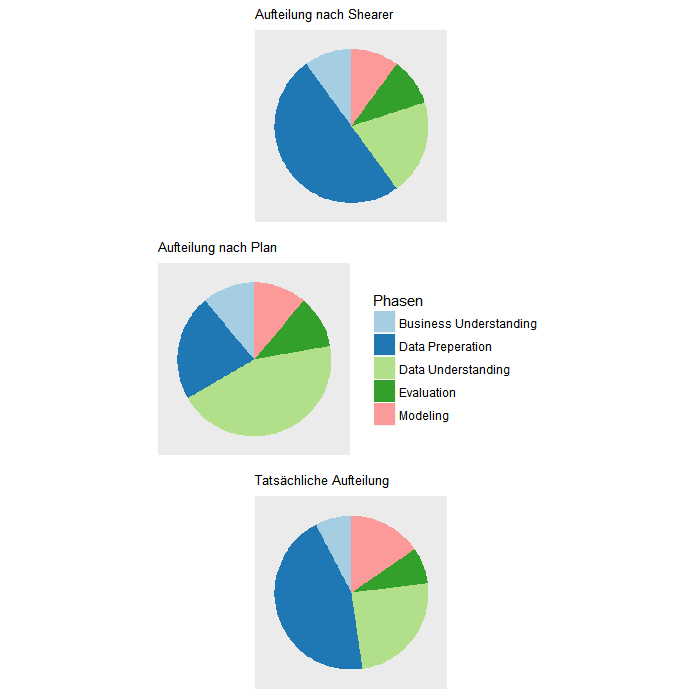
\includegraphics[width=\textwidth]{images/phases2}}
\caption{Tortendiagramme des Projektaufwands nach Shearer, nach Plan und des tatsächlicher Aufwands}
\label{fig:phases}
\end{figure}

\subsection{Umgang mit den Erkenntnissen (Determine Next Steps)}
Im Referenzmodell folgt nach der Evaluation das Deployment. Im Falle dieser Untersuchung wird jedoch darauf verzichtet. Einerseits besitzen die erstellten Modelle noch nicht den Reifegrad, um genutzt zu werden, andererseits würde der Aufwand den Umfang der Arbeit übersteigen.
Im weiteren wird wie oben (Punkt \ref{subsec:revRes}) angesprochen, das Werkzeug Azure Machine Learning Studio bewertet (Punkt \ref{sec:BeswertungAzure}), eine Aussage über das Referenzmodell CRIPS-DM getroffen (Punkt \ref{sec:BeswertungCrisp}) und die Ergebnisse des Machine Learning interpretiert (Punkt \ref{sec:BewertungML}).




